\chapter[Proposal]{Proposal}
\label{chap:proposal}

This proposal focuses on detailing the necessary steps to the creation and publication of a crowdfunding speech corpus in Brazilian Portuguese. To this end, a virtual voice recording application will be developed (section \ref{sec:proposal-app}), focusing on adding gamification elements to enhance user engagement. Additionally, this application will also extract some relevant speaker characteristics found in the systematic literature review in chapter \ref{chap:slr}, such as speaker demographics. Once the construction is finished, the application will be released, allowing general public submission (in section \ref{sec:proposal-public-submission}). After the submission period, the collected data will be analyzed and compiled to a speech corpus (\ref{sec:proposal-data-analysis}), which will be publicized to an open-source repository in section \ref{sec:proposal-data-publication}.

\section{Application}
\label{sec:proposal-app}

This section details the conception, documentation, and development process of the voice recording application, coined "Fale Alguma Coisa". Below, it will at times be referenced as "app", or "WebApp", short for Application and Web Application, respectively. The main purpose of this app is to be able to record predetermined phrases from users. All other features support the engagement and usability through authentication, gamification, and explanatory elements. The following documentation structure is based on Pressman's book "Software Engineering: A Practitioner's Approach" \cite{pressman2014software}, and generated a proper Software Requirements Specification in the Appendix \ref{appendix:srs}. Hence, some details will be omitted to provide simplicity and overall understanding of the design process.

In this simplified explanation, the scope will be detailed \ref{sec:app-scope}, followed by the artefacts produced \ref{sec:app-artefacts}. Secondly, the functionality of the entire application will be documented using use cases (\ref{sec:simplified-use-cases}). Next, the navigation structure of some use cases will be documented (\ref{sec:navigation-design}), followed by the aesthetic design (in \ref{sec:aesthetic-design}). Then, the user interface will be elaborated by documenting the layouts (in \ref{sec:app-user-interface}), based on the use cases listed and previous decisions. One key factor in the app is the ability to teach science facts and trivia, which entails the need of proper phrase selection methods. These methods will be explained in the section \ref{sec:app-phrase-selection}. Lastly, the development process will be described, with additional details on the tools selected (\ref{sec:app-development}). Again, many steps of the software design process were skipped in this proposal, but a thorough description can be referred to in Appendix \ref{appendix:srs}.

\begin{figure}[ht]
    \centering
    \caption{Fale Alguma Coisa app Logo}
     
\includegraphics[width=\linewidth/2]{images/app/logo.jpg}
    \caption*{Source: Author}
    \label{fig:falealgumacoisa-logo}
\end{figure}

\subsection{Scope}
\label{sec:app-scope}

Towards contributing \textbf{nonprofessional scientists}, the Fale Alguma Coisa app should provide an easy gateway for the user to contribute his voice while having fun and learning various science facts and curiosities.

Towards researching \textbf{scientists}, the Fale Alguma Coisa app should provide a database of anonymized voice recordings for scientists to extract and create a speech corpus.

Directed towards anyone interested in learning and contributing to science.

\subsubsection{Outside scope}

However, some elements are outside of the scope of this system. These elements are clarified in this section, as Fale Alguma Coisa should \textbf{not}:
\begin{itemize}
    \item allow for association of recording data and personal identification data (name, email);
    \item support internationalization in the WebApp;
    \item convert audio data into another format;
    \item support offline recording.
\end{itemize}

\subsection{Artefacts}
\label{sec:app-artefacts}

This table presents the artefacts to be produced, and their respective locations in this work.

\begin{table}[h]
\centering
\caption{Artefacts produced by the specification and their respective locations}
\label{tab:artifact-locations}
\begin{tabular}{|p{3.5cm}|p{2.5cm}|p{9cm}|}
    \hline 
    Artefact & Location & Description \\ \hline 
    Purpose & Appendix \ref{appendix:purpose} & Defines the purpose of the Software Requirements Specification documentation \\ \hline
    Scope & Appendix \ref{appendix:scope} & Artefacts, Objectives, Out of Scope \\ \hline
    System Overview & Appendix \ref{appendix:system-overview} & Project perspective, System Context, General Constraints, Assumptions and Dependencies \\ \hline
    Actor List & Appendix \ref{appendix:actor-list} & List of actors involved with the system \\ \hline 
    Simplified Requirements & Section \ref{sec-simplified-use-cases} & Simplified use cases \\ \hline
    Scenario-based Models & Appendix \ref{appendix:scenario-based-model} & Detailed use cases \\ \hline
    Class Models & Appendix \ref{appendix:domain-model} & Class diagrams to model the domain of the system, mapping relationship and collaboration \\ \hline
    Behavior Models & Appendix \ref{appendix:behavior-model} & State and sequence diagrams to fully document specific and more complex behavior \\ \hline
    Non-Function Requirements & Appendix \ref{appendix:non-fuctional-requirements} & i.e.: Usability, Performance, Security, Legal, Requirements, etc. \\ \hline
    Interface Requirements & Appendix \ref{appendix:interface-requirements} & Machine and External Systems interfaces \\ \hline
    Navigation Design & Appendix \ref{appendix:navigation-design} & Navigation Semantic Units \\ \hline
    User Interface Design & Appendix \ref{appendix:user-interface-design} & For each use case, a user interface will be developed and documented \\ \hline
    Application Architecture & Appendix \ref{appendix:architecture} & Before WebApp must have  \\ \hline
    Tools and Frameworks Selection & Appendix \ref{appendix:tools-selection} & To develop the documented application, a set of tools and frameworks shall be selected \\ \hline
    FaleAlgumaCoisa WebApp & Appendix \ref{appendix:webapp} & Description of developed web application \\ \hline
    FaleAlgumaCoisa Backend & Appendix \ref{appendix:backend} & Description of developed backend application \\ \hline
\end{tabular}
\caption*{Source: Author}
\end{table}

\clearpage
\subsection{Use Cases}
\label{sec:simplified-use-cases}

A simplified list of use cases is reproduced in the following tables (\ref{tab:falealgumacoisa-simplified-home}, \ref{tab:falealgumacoisa-simplified-recording}, \ref{tab:falealgumacoisa-simplified-dashboard}, \ref{tab:falealgumacoisa-simplified-social}, \ref{tab:falealgumacoisa-simplified-gamification}, \ref{tab:falealgumacoisa-simplified-login-and-registration}) below, separated by feature set. To a more complete specification, refer to section \ref{appendix:use-cases} in the Appendix.

\subsubsection{Home}

In table \ref{tab:falealgumacoisa-simplified-home}, use cases affecting the homepage are listed, such as the splash screen, project description, navigation, and terms of service.

\begin{table}[h]
\caption{Simplified Home Use Cases for the Fale Alguma Coisa WebApp}
\label{tab:falealgumacoisa-simplified-home}
\centering
\begin{tabular}{|p{1cm}|p{3cm}|p{10cm}|}
\hline
    Code & Use Case Name & Description \\ \hline
    UC01 & View Home Splash & An unregistered citizen wants to view an animated introductory screen (splash) when entering the application, so that he feels more inside a native app. \\ \hline
    UC02 & View Home Description & An unregistered citizen wants to check the initiative description, so that he understands more about the Fale Alguma Coisa citizen science project. \\ \hline
    UC03 & Navigate Home Login & A registered citizen wants to navigates from the homepage to the sign-in page, so that he logins (or register) to his account. \\ \hline
    UC04 & Navigate Home Recording & An unregistered citizen wants to easily navigate from the homepage to the recording page, so that he can contribute his voice. \\ \hline
    UC05 & Read Home Terms & An unregistered citizen wants to reads the terms of service (and privacy policy) of Fale Alguma Coisa, so that he understands better what the service has to offer and what kind of data will be recorded. \\ \hline
\end{tabular}
\caption*{Source: Author}
\end{table}

\clearpage
\subsubsection{Recording}

Represents the most important feature in the application, as the citizen will use it to record his voice. It also provides supporting features, such as skipping phrases and resuming the recording session. The list of simplified use cases is listed in table \ref{tab:falealgumacoisa-simplified-recording}; with the complete version available in Appendix \ref{appendix:scenario-based-model}

\begin{table}[h]
\caption{Simplified Recording Use Cases for the Fale Alguma Coisa WebApp}
\label{tab:falealgumacoisa-simplified-recording}
\centering
\begin{tabular}{|p{1cm}|p{3cm}|p{10cm}|}
\hline
    Code & Use Case Name & Description \\ \hline
    UC10 & Accept Terms & An unregistered citizen would like to view and accept the terms of service before recording, so that he understands how his data is being used. \\ \hline
    UC11 & Configure Microphone & An unregistered citizen would like to properly configure my microphone before recording, so that he can record without interruption. \\ \hline
    UC12 & Record Phrases & A citizen would like to read science phrases with definitions and curiosities, so that he learns about subjects as he is contributing. \\ \hline
    UC13 & Group Phrases & A citizen would like to read phrases grouped by theme, so that he can learn more from each subject as he is contributing. To finish a theme, the citizen must read 6 phrases. \\ \hline
    UC14 & Read Tutorial & A citizen would like to read a tutorial explaining how to record, so that he learns how to properly record phrases. \\ \hline
    UC15 & Watch Recording Animations & A citizen would like to see animations on each step of the recording (enter the page, start the recording, stop the recording), so that he feels more engaged with the application. \\ \hline
    UC16 & Skip Phrase & A citizen would like to skip a phrase when he (1) does not know how to pronounce, or (2) finds a foreign word, or (3) finds another specified reason, so that he only speaks the correct phrases. A maximum of 2 skips are allowed. \\ \hline
    UC17 & Stop Recording Session & A citizen would like to stop this recording session by clicking the logo and confirming the exit, so that he can resume it afterwards. \\ \hline
\end{tabular}
\caption*{Source: Author}
\end{table}

\clearpage
\subsubsection{Dashboard}

Table \ref{tab:falealgumacoisa-simplified-dashboard} lists all user stories related to the dashboard page, such as where the user will be able to choose themes to record, open the menu, check his level, etc.

\begin{table}[h]
\caption{Simplified Dashboard Use Cases for the Fale Alguma Coisa WebApp}
\label{tab:falealgumacoisa-simplified-dashboard}
\centering
\begin{tabular}{|p{1cm}|p{3cm}|p{10cm}|}
\hline
    Code & Use Case Name & Description \\ \hline
    US20 & Navigate Register & An unregistered citizen would like to easily register his data through a button click, so that he can enjoy all features of the logged area. \\ \hline
    US21 & View Actions & A registered citizen would like to see his actions in a dashboard after logging in, so that he can better contribute to the project. \\ \hline
    US22 & Recommend Themes & A registered citizen would like to see a list of recommended themes to speak, so that he can choose one from the list. \\ \hline
    US23 & View Progress Level & A registered citizen would like to view my progress level, so that he know how far have he  progressed in my contributions. \\ \hline
    US24 & Open Menu & A registered citizen would like to open the menu, so that he knows which are his possible actions in the app. \\ \hline
    US25 & View Notifications & A registered citizen would like to check notifications, so that he understands what happened while he was gone. \\ \hline
\end{tabular}
\caption*{Source: Author}
\end{table}

\subsubsection{Social}

To allow the social interaction with other users, the table \ref{tab:falealgumacoisa-simplified-social} lists social use cases to be added to the application. Not all social interaction is listed in this feature, as there are some elements in gamification, such as competition.

\begin{table}[h]
\caption{Simplified Social Use Cases for the Fale Alguma Coisa WebApp}
\label{tab:falealgumacoisa-simplified-social}
\centering
\begin{tabular}{|p{1cm}|p{3cm}|p{10cm}|}
\hline
    Code & Use Case Name & Description \\ \hline
    US30 & Add Friend & A registered citizen would like to add a friend, so that he can check them in the friends leaderboard afterwards. \\ \hline
    US31 & View Notifications & A registered citizen would like to check notifications, so that he can know what happened when he was away. \\ \hline
    US32 & Receive Notifications & A registered citizen would like to know when someone added him through notifications, so that he can add them back later. \\ \hline
    US33 & Refer Friends & A registered citizen would like to refer friends to the application, so that he can play with them afterwards. \\ \hline
\end{tabular}
\caption*{Source: Author}
\end{table}

\subsubsection{Gamification}

Table \ref{tab:falealgumacoisa-simplified-gamification} details the engagement component of the application. Elements such as leaderboards, points and levels are described. They add competition and a sense of progress to the user experience, supporting the core need of this system, which is phrase recording.

\begin{table}[h]
\caption{Simplified Gamification Use Cases for the Fale Alguma Coisa WebApp}
\label{tab:falealgumacoisa-simplified-gamification}
\centering
\begin{tabular}{|p{1cm}|p{3cm}|p{10cm}|}
\hline
    Code & Use Case Name & Description \\ \hline
    US40 & Earn First Recording & A registered citizen would like to get 100 points when he records his first phrase, so that he can engage better in the application. \\ \hline
    US41 & Earn First Theme & A registered citizen would like to get 400 points when he records his first theme, so that he can engage better in the application. \\ \hline
    US42 & Earn Theme & A registered citizen would like to get 300 points when he records subsequent themes, so that he can engage better in the application. \\ \hline
    US43 & Earn Registration & A registered citizen would like to get 500 points when he registers his speaker data, so that he can better engage with the application. \\ \hline
    US44 & Calculate Level & A registered citizen would like to measure his points through a level, so that he can more easily compare himself with other users. \\ \hline
    US45 & Compete Top Players & A registered citizen would like to know who are the top contributors in the space and where he is in the list, so that he can compete against them. \\ \hline
    US46 & Compete Friends & A registered citizen would like to know where his friends are in the friends leaderboard, so that he can compete against them. \\ \hline
\end{tabular}
\caption*{Source: Author}
\end{table}

\subsubsection{Login and Registration}

The application should provide user authentication to enable data management and progress saving. Table \ref{tab:falealgumacoisa-simplified-login-and-registration} lists all use cases referring to this feature, and is the key to generating recordings with speaker metadata.

\begin{table}[h]
\caption{User Stories categorized to the login and registration epic for the Fale Alguma Coisa WebApp}
\label{tab:falealgumacoisa-simplified-login-and-registration}
\centering
\begin{tabular}{|p{1cm}|p{3cm}|p{10cm}|}
\hline
    Code & Use Case Name & Description \\ \hline
    US50 & Login Social & An unregistered citizen would like to login (using social login - Facebook / Google) on the app, so that he can login later and save my progress. \\ \hline
    US51 & Register Metadata & A unregistered citizen would like to register his anonymous data on his first login, so that he can provide better metadata to my recordings afterwards. \\ \hline
    US52 & Update Account & A registered citizen would like to update his account data, so that he can provide accurate metadata on the recordings. \\ \hline
    US53 & Delete Account & A registered citizen would like to remove his account data (and his recordings, if necessary), so that he can remove my metadata from this application. \\ \hline
\end{tabular}
\caption*{Source: Author}
\end{table}

\clearpage
\subsection{Navigation Design}
\label{sec:navigation-design}

Ensuring a robust navigation design for the user enables him to access the WebApp contents and functions. To accomplish this, it is necessary to: (1) identify the semantics of navigation for different users, and (2) define the mechanics of achieving the navigation. They are defined by a series of \textit{navigation semantic units} (NSUs), a set of information and related navigation structures that collaborate in the fulfillment of a subset of related user requirements \cite{conallen2003building}.

\subsubsection{Navigational Semantics}

A NSU is composed of a set of navigation elements called \textit{ways of navigating} (WoN). A WoN represents the the best navigation pathway to achieve a navigational goal for a specific type of user. Each WoN is organized as a set of \textit{navigational nodes} (NN) that are connected by navigational links. An example of NSU is given below in figure \ref{fig:app-nsu-example}.

\begin{figure}[h]
    \centering
    \caption{Navigation Semantic Unit for an Unregistered User Recording}
    \label{fig:app-nsu-example}
    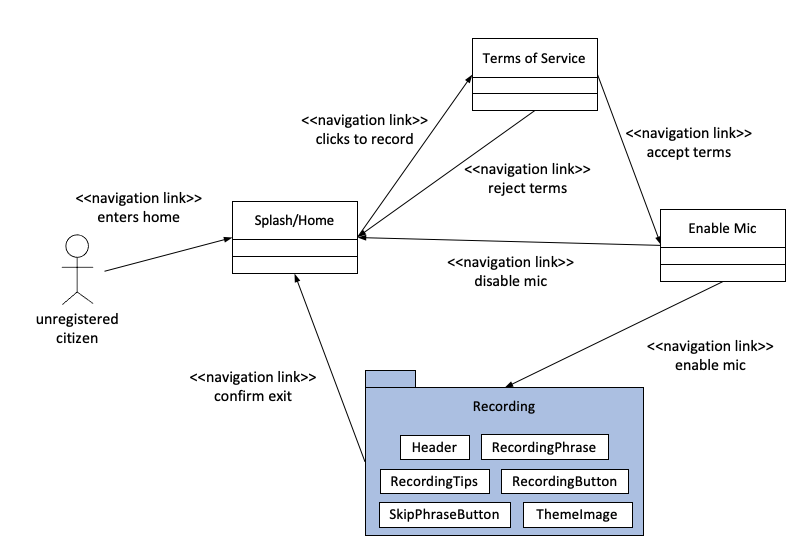
\includegraphics[width=\linewidth]{images/sw-req-spec/nsu-unregistered.png}
    \caption*{Source: Author}
\end{figure}

In figure \ref{fig:app-nsu-example}, the navigation behavior to record a phrase of an unregistered user is illustrated. As the unregistered user enters the homepage, he clicks the start recording button. However, since he has neither accepted the terms of service nor enabled his microphone permission, he must go through these pages. If he denies the terms or microphone permission, he is redirected to the homepage. If the user allows both, he will enter the recording page, where he is able to record phrases and donate his voice.

This is only one example of the more complex user Ways of Navigations. Refer to appendix \ref{appendix:navigation-design} to a more complete list of NSUs.

\subsection{Aesthetic Design}
\label{sec:aesthetic-design}

To reference some aesthetic design guidelines from \cite{pressman2014software}:

\begin{itemize}
    \item Emphasize content;
    \item Organize layout elements from top left to bottom right;
    \item Group navigation, content, and function geographically within the page;
    \item Do not extend your real state with the scrolling bar;
    \item Consider resolution and browser window size when designing layout.
\end{itemize}

\subsubsection{Color Scheme}

In color theory, colors are used to communicate meaning, but also affect mood, and perception \cite{agoston2013color}. The design color scheme defines a color palette to choose from when designing new visual elements. Applying this concept, a colorful color scheme was chosen to lighten the mood of the application, as shown in figure \ref{fig:falealgumacoisa-color-scheme}.

\begin{figure}[h]
    \centering
    \caption{Fale Alguma Coisa color scheme}
     
\includegraphics[width=.5\linewidth]{images/app/colors.png}
    \caption*{Source: Author}
    \label{fig:falealgumacoisa-color-scheme}
\end{figure}

\subsection{User Interface}
\label{sec:app-user-interface}

To ensure an effective development of the user interface, an iterative analysis and design approach was taken \cite{pressman2014software}. This design process is illustrated in figure \ref{fig:user-interface-design-process}, and emcompasses four distinct framework activities: (1) interface analysis and modeling, (2) interface design, (3) interface construction, and (4) interface validation. The spire implies that each of these tasks will occur more than once, with each pass around the spiral representing an additional elaboration of requirements and the resultant design. The user interface hereby implemented is the outcome of many of these iterations, with each major use case implemented into a finalized artefact. For an extensive list, refer to the Appendix \ref{appendix:user-interface-design}.

\begin{figure}[h]
    \centering
    \caption{The user interface design process}
    \label{fig:user-interface-design-process}
    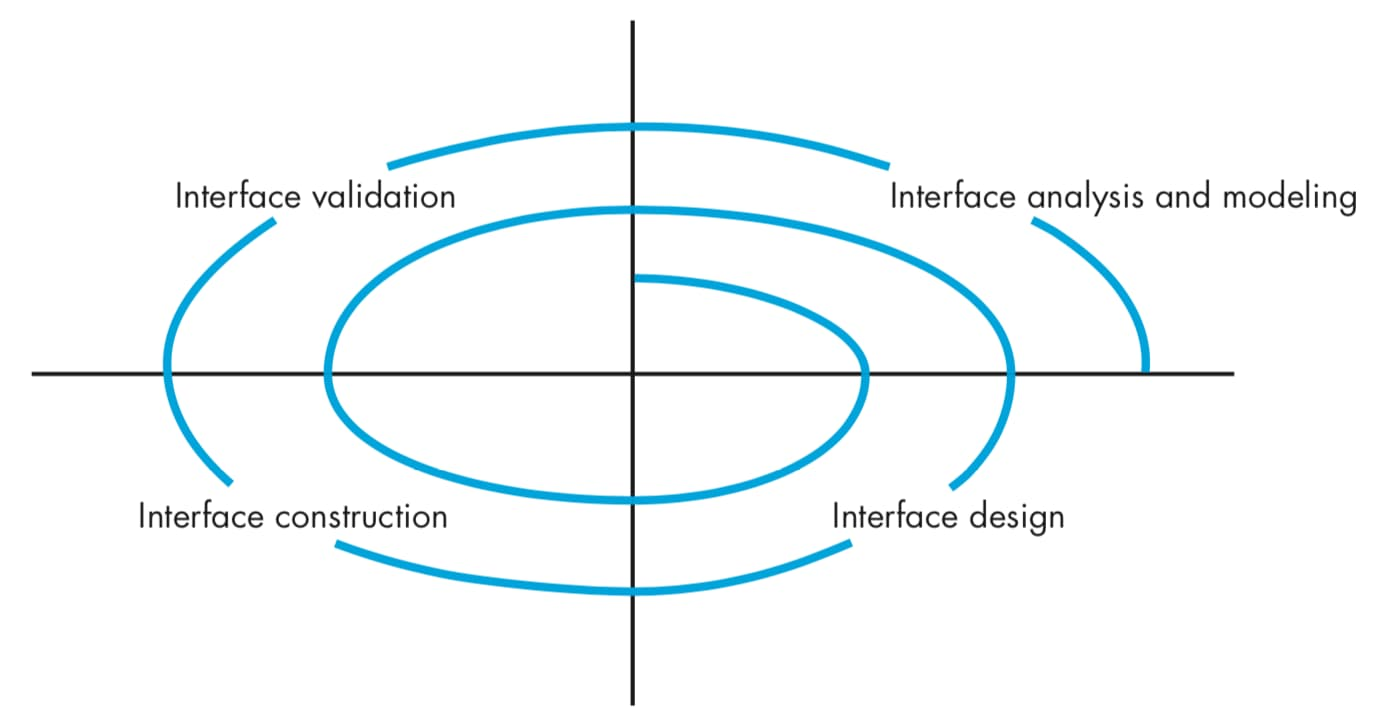
\includegraphics[width=.8\linewidth]{images/sw-req-spec/user-interface-design-process.jpg}
    \caption*{Source: \cite{pressman2014software}}
\end{figure}

\clearpage
\subsubsection{Splash Screen}

As the user first enter the application, a splash screen will be shown to welcome him (mobile version in figure \ref{fig:falealgumacoisa-splash-page-design}). It contains the logo and an animation to draw the user's attention. After the animation, the home will be shown.

\begin{figure}[ht]
    \centering
    \caption{Fale Alguma Coisa Splash Page design}
    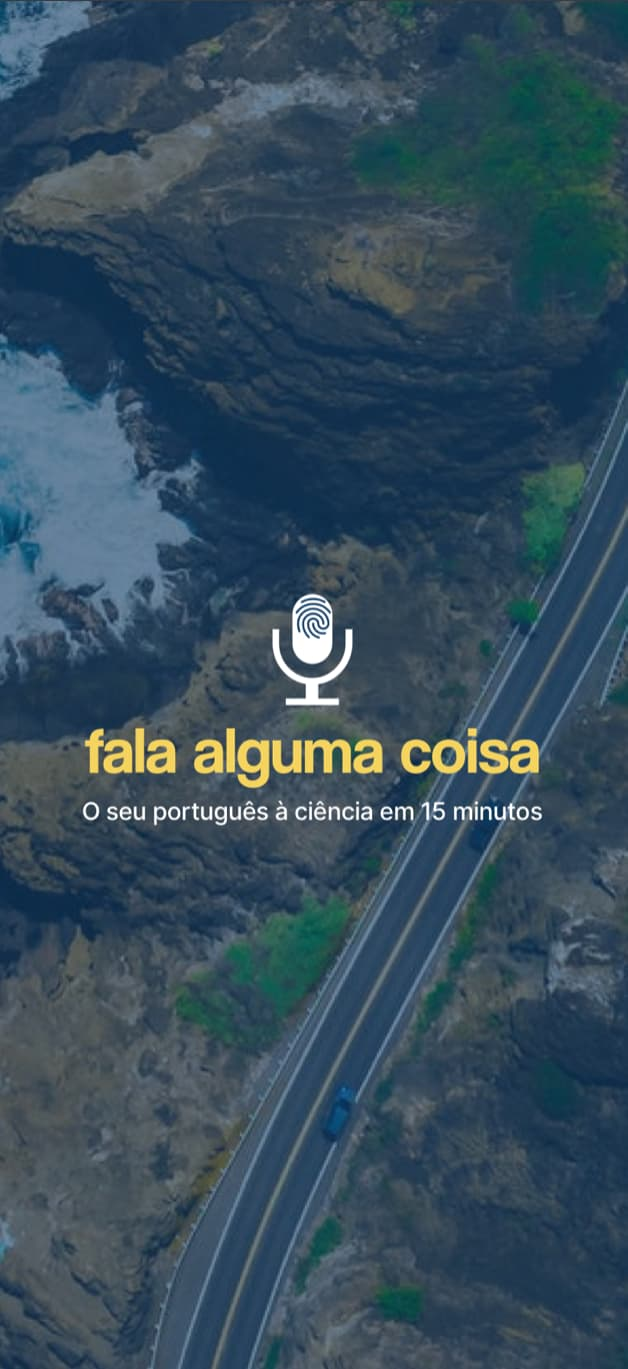
\includegraphics[width=\linewidth/2]{images/app/m-splash.jpg}
    \caption*{Source: Author}
    \label{fig:falealgumacoisa-splash-page-design}
\end{figure}

\subsubsection{Homepage}

After the splash animation, the homepage is shown. The mobile version can be seen below in figure \ref{fig:falealgumacoisa-home-page-design}. In this page, the call to action to start the recording is highlighted by the button at the center of the page, with text describing the project right below it. The login page is accessible through the link in the right upper corner. These few elements are placed to encourage the user to click on the recording, if he is a new user.

\begin{figure}[ht]
    \centering
    \caption{Fale Alguma Coisa Home Page design}
    \frame{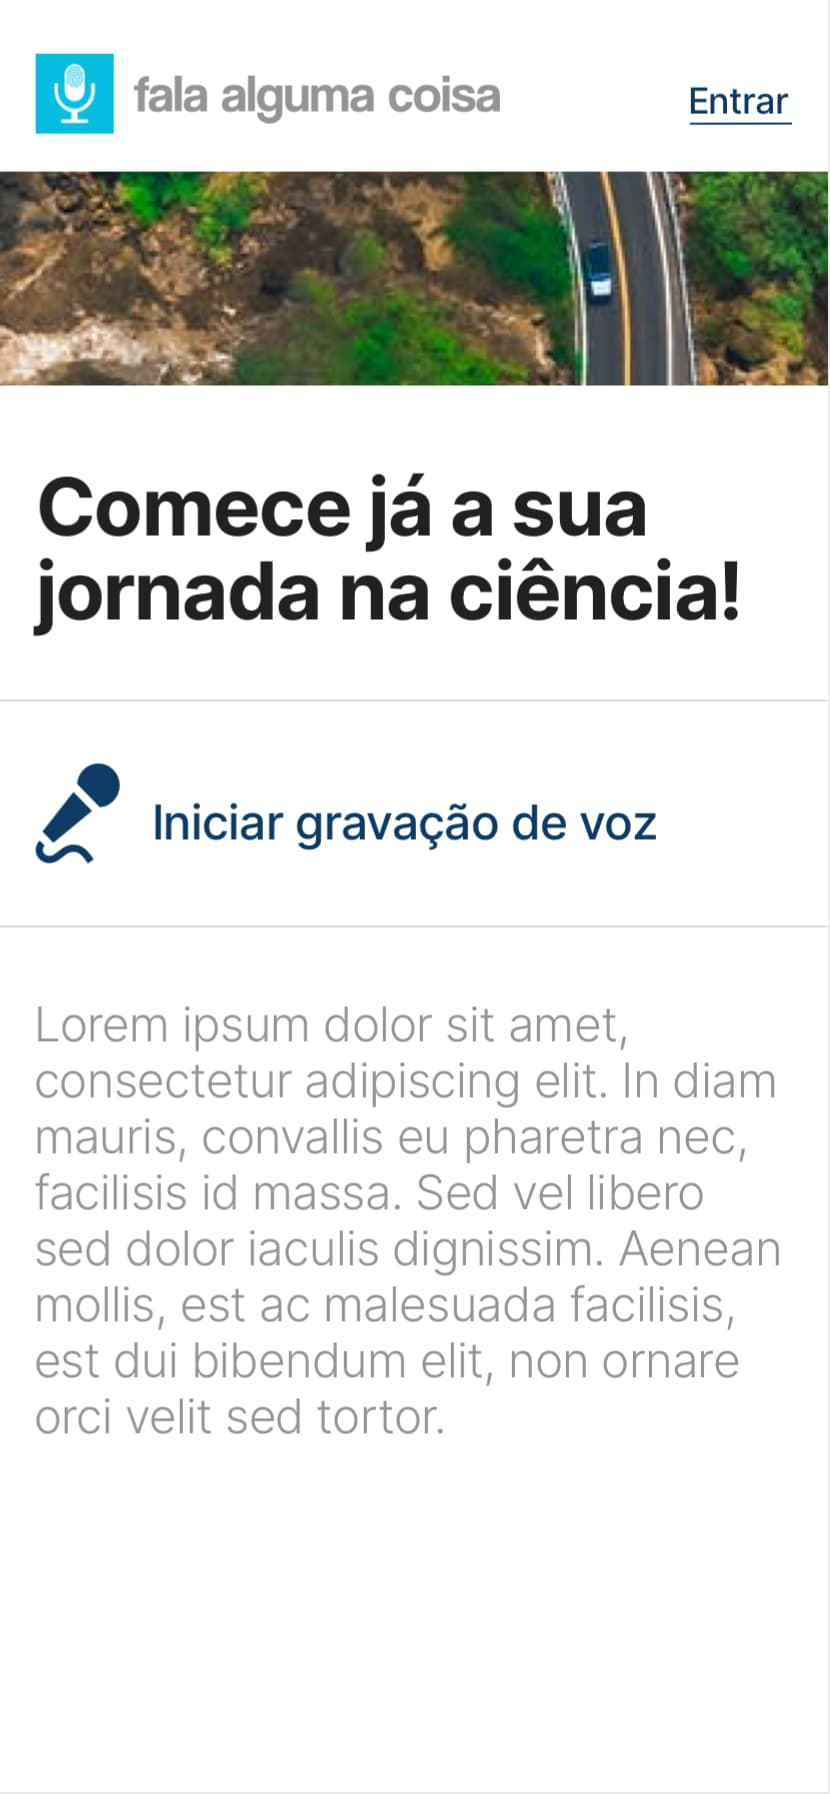
\includegraphics[width=\linewidth/2]{images/app/m-home.jpg}}
    \caption*{Source: Author}
    \label{fig:falealgumacoisa-home-page-design}
\end{figure}

\subsubsection{Recording}

This page represents the core functionality of the website, allowing the user to record phrases with his voice. The recording is done through groups of phrases, called a theme, and is illustrated by the image \ref{fig:falealgumacoisa-recording-page-design} at the bottom. The main elements of the page are (1) the phrase highlighted in a rectangular box at the center of the page, and (2) the red recording button at the bottom.

\begin{figure}[ht]
    \centering
    \caption{Fale Alguma Coisa Recording Page designs}
    \begin{subfigure}{.5\textwidth}
      \centering
      \frame{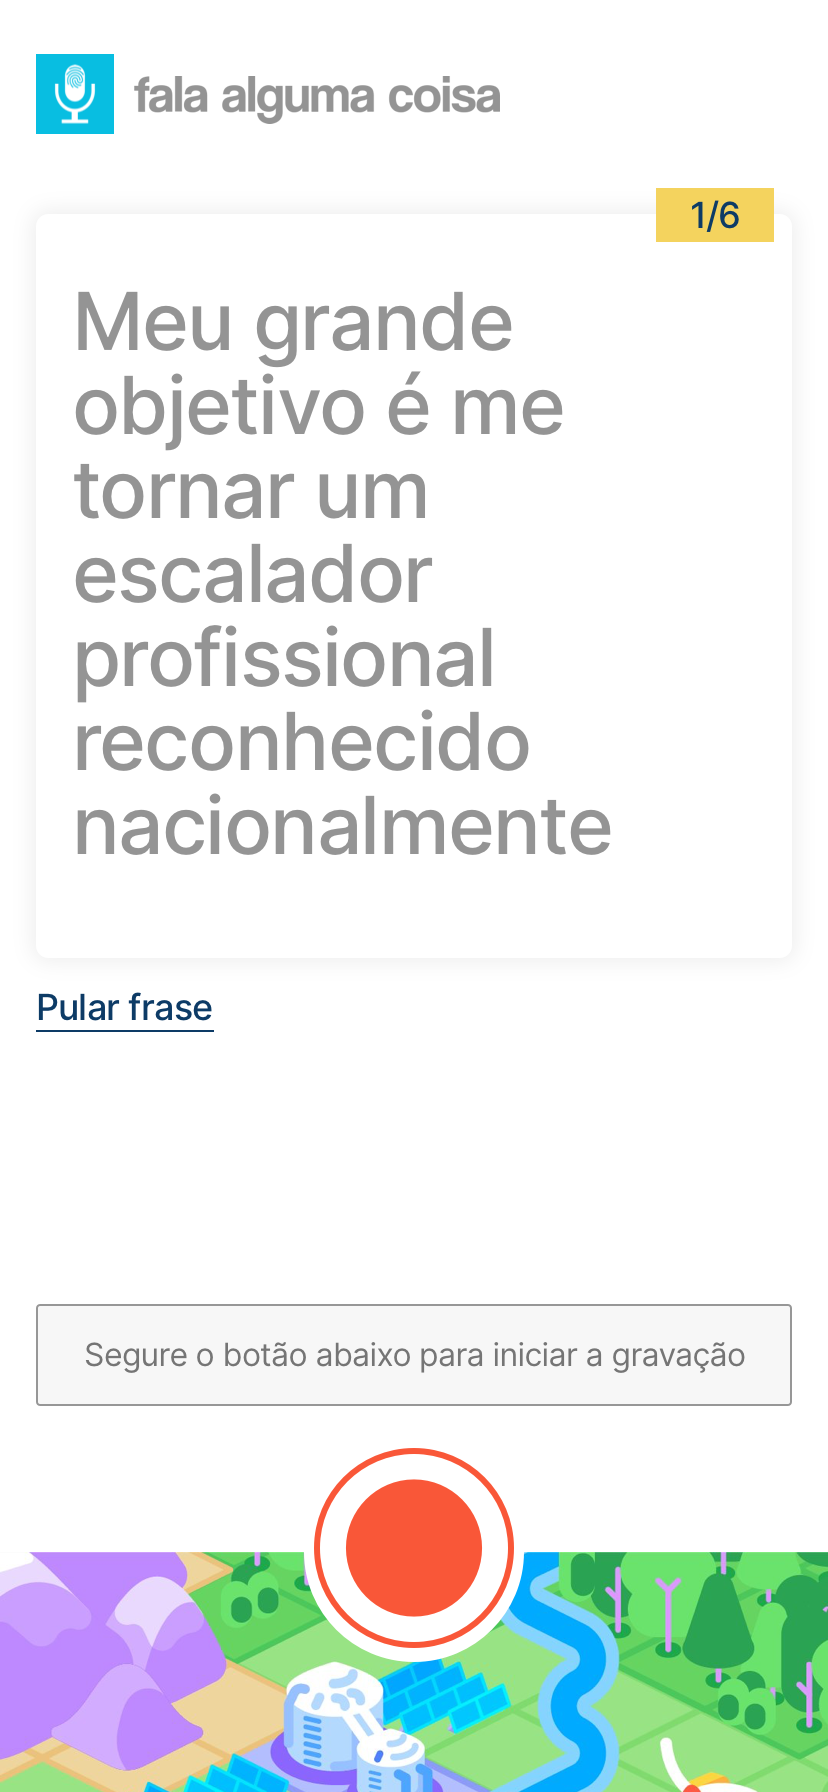
\includegraphics[width=.9\linewidth]{images/app/recording/Journey_1.0.png}}
      \caption{Waiting to start recording}
      \label{fig:falealgumacoisa-recording-page-design-start}
    \end{subfigure}%
    \begin{subfigure}{.5\textwidth}
      \centering
      \frame{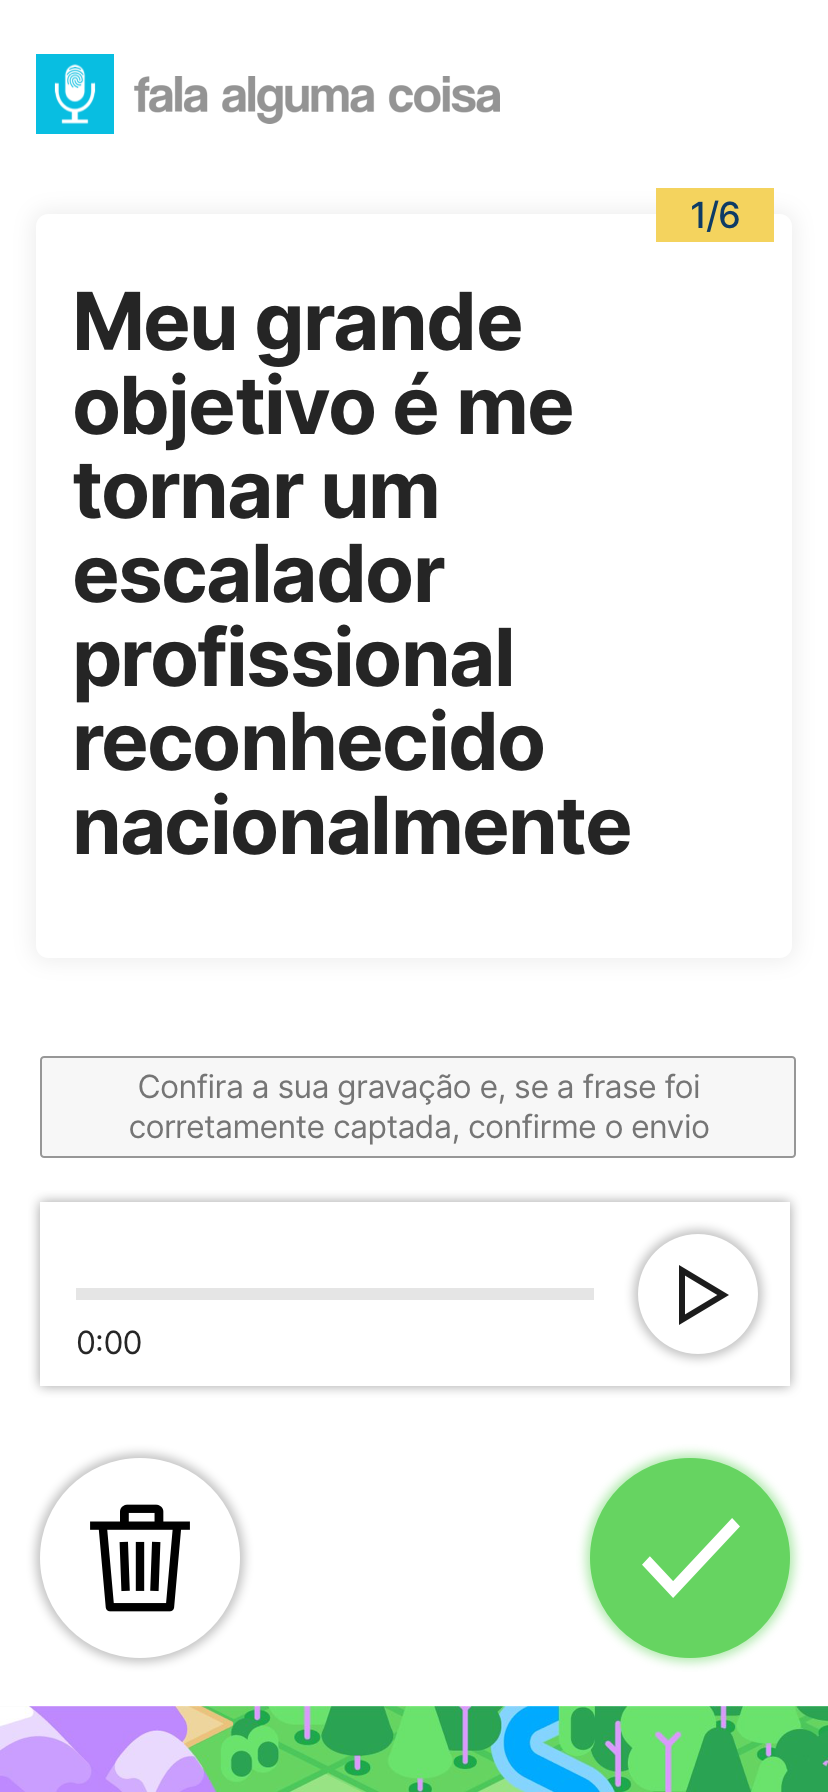
\includegraphics[width=.9\linewidth]{images/app/recording/Journey_1.2.png}}
      \caption{Confirm or delete recording}
      \label{fig:falealgumacoisa-recording-page-design-confirm}
    \end{subfigure}
    \caption*{Source: Author}
    \label{fig:falealgumacoisa-recording-page-design}
\end{figure}

\subsubsection{Terms of Service}

To comply with Brazil's General Data Protection Act (Law 13,709/2018), the application has to clarify data usage of the visitor of the website. The figure \ref{fig:falealgumacoisa-tos-page-design} defines the layout of the page with a simplified terms of service, as well as a button to accept or deny such terms.

\begin{figure}[ht]
    \centering
    \caption{Fale Alguma Coisa simplified terms of service page design}
    \frame{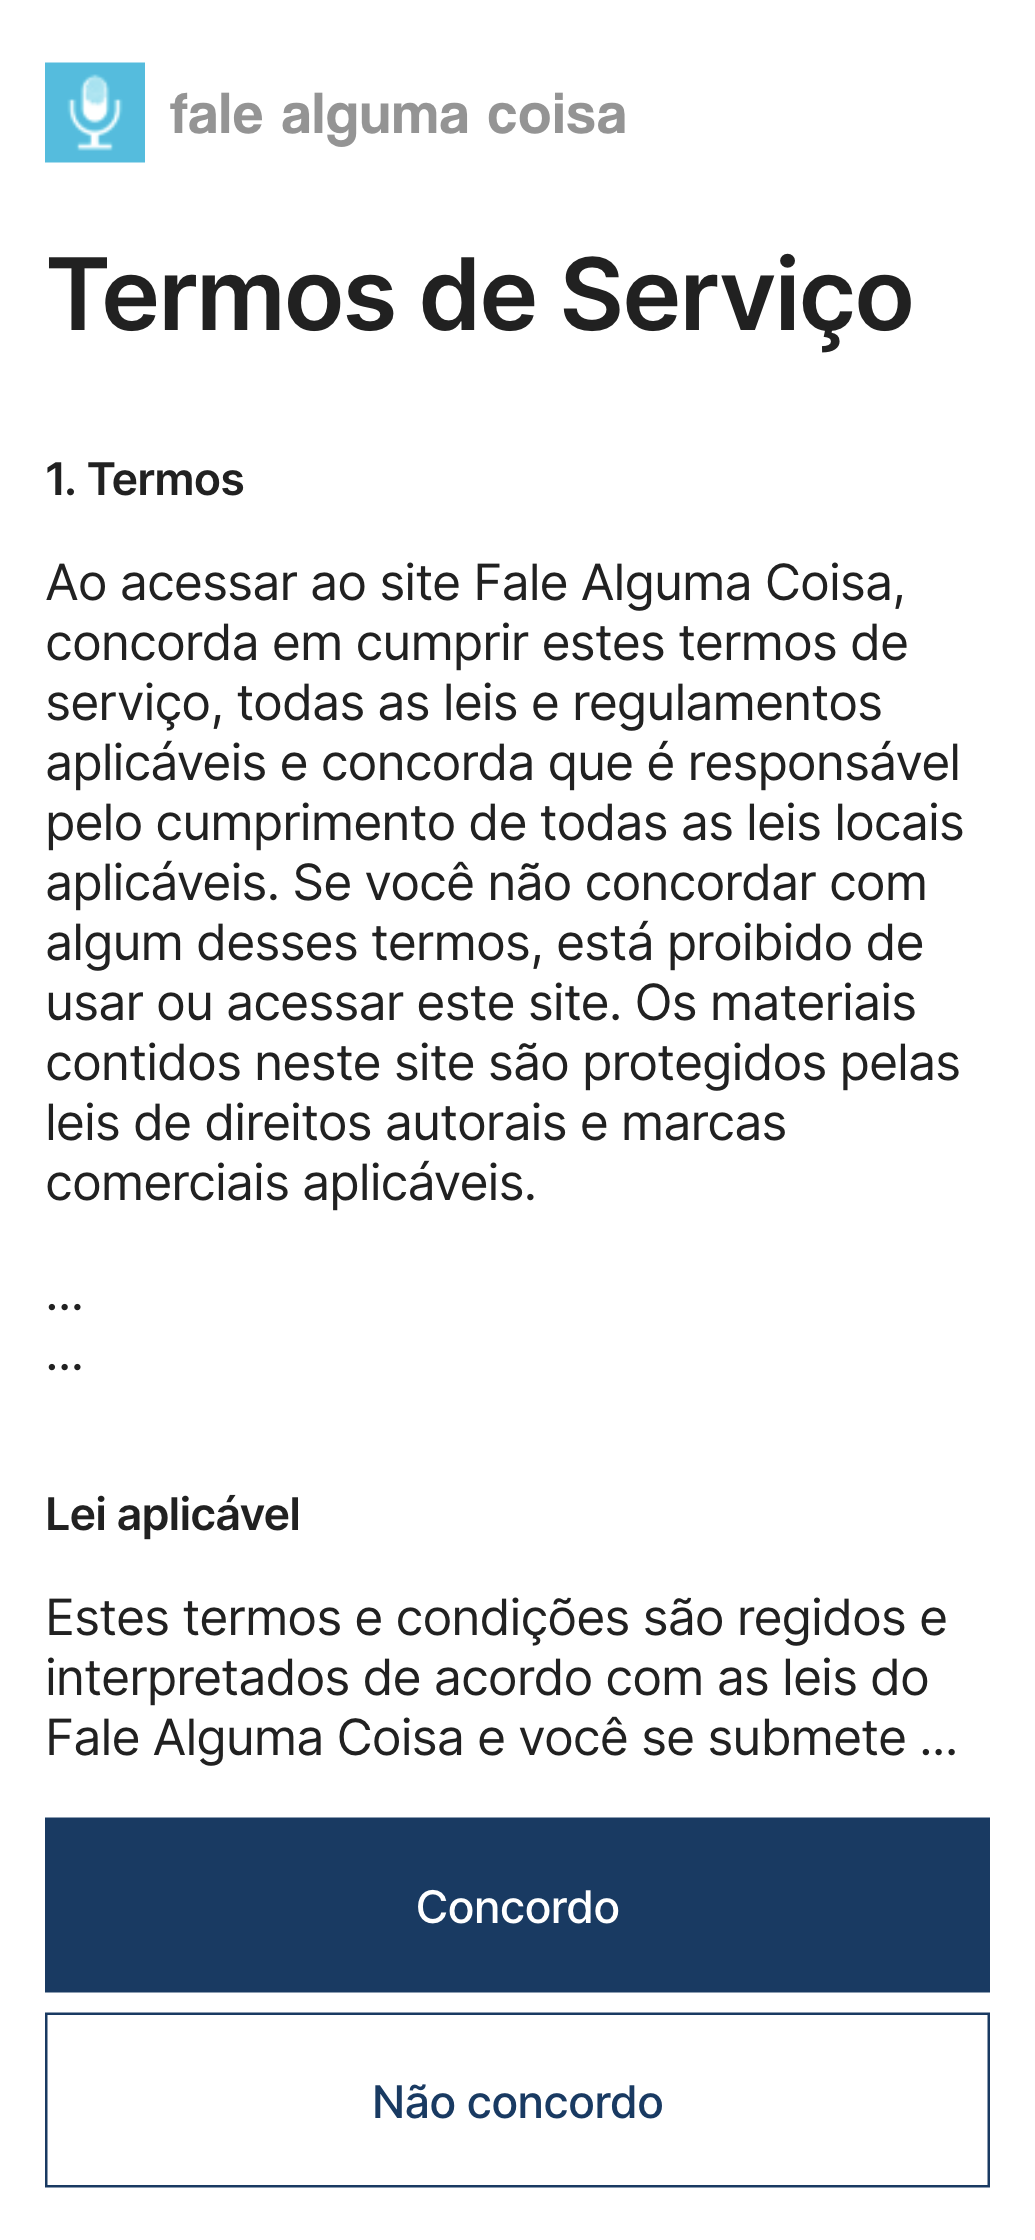
\includegraphics[width=\linewidth/2]{images/app/register/tos.png}}
    \caption*{Source: Author}
    \label{fig:falealgumacoisa-tos-page-design}
\end{figure}

\subsubsection{Dashboard}

When an unauthenticated user finishes recording its first theme, or when a user logs in, they are able to select from a list of themes to record. In this dashboard seen in figure \ref{fig:falealgumacoisa-dashboard-page-design}, they are also shown the number of points accumulated by the usage of the app, as well as able to open a menu and notification page.

\begin{figure}[ht]
    \centering
    \caption{Fale Alguma Coisa Dashboard Page design}
    \frame{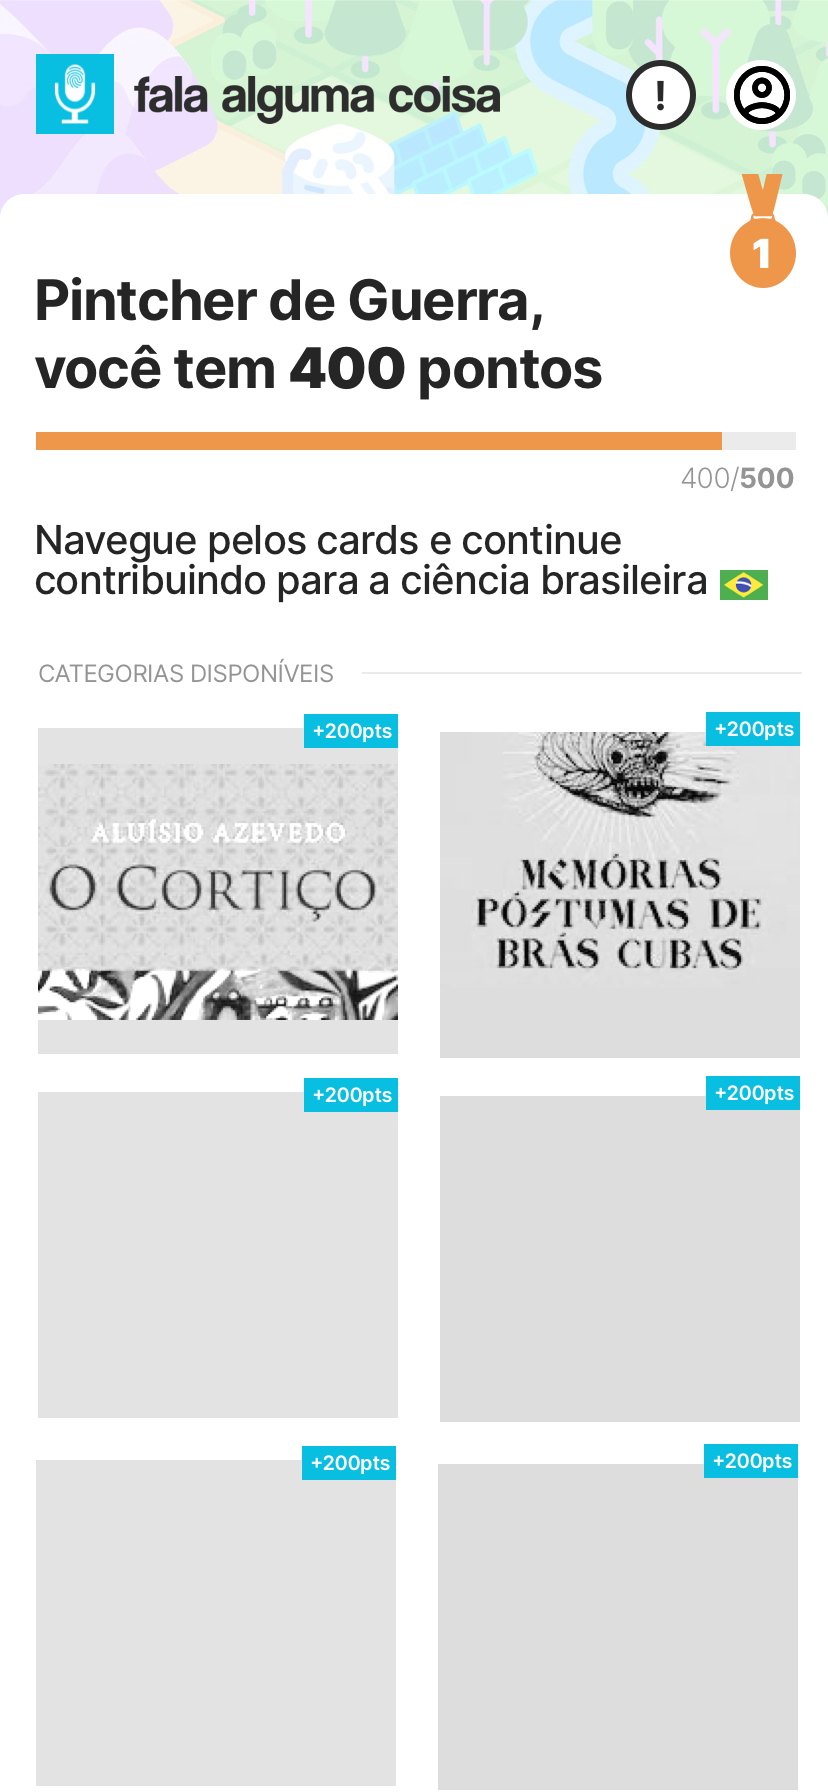
\includegraphics[width=\linewidth/2]{images/app/dashboard/Dashboard.png}}
    \caption*{Source: Author}
    \label{fig:falealgumacoisa-dashboard-page-design}
\end{figure}

\subsubsection{Leaderboard}

The leaderboard layouts feature two visualizations, depending on the desired scope. Should the contributor want to see all top ranking users, the leaderboard (figure \ref{fig:falealgumacoisa-leaderboard-page-design-general}) is available. If the user only wants to check his friend rankings, the application displays a reduced list (figure \ref{fig:falealgumacoisa-leaderboard-page-design-friend}), based on the friends added to the platform. These layouts provide a way for users to compare their contributions, thus promoting competition. A social element is also included throughout the option to add friends.

\begin{figure}[ht]
    \centering
    \caption{Fale Alguma Coisa Leaderboard Page designs}
    \begin{subfigure}{.5\textwidth}
      \centering
      \frame{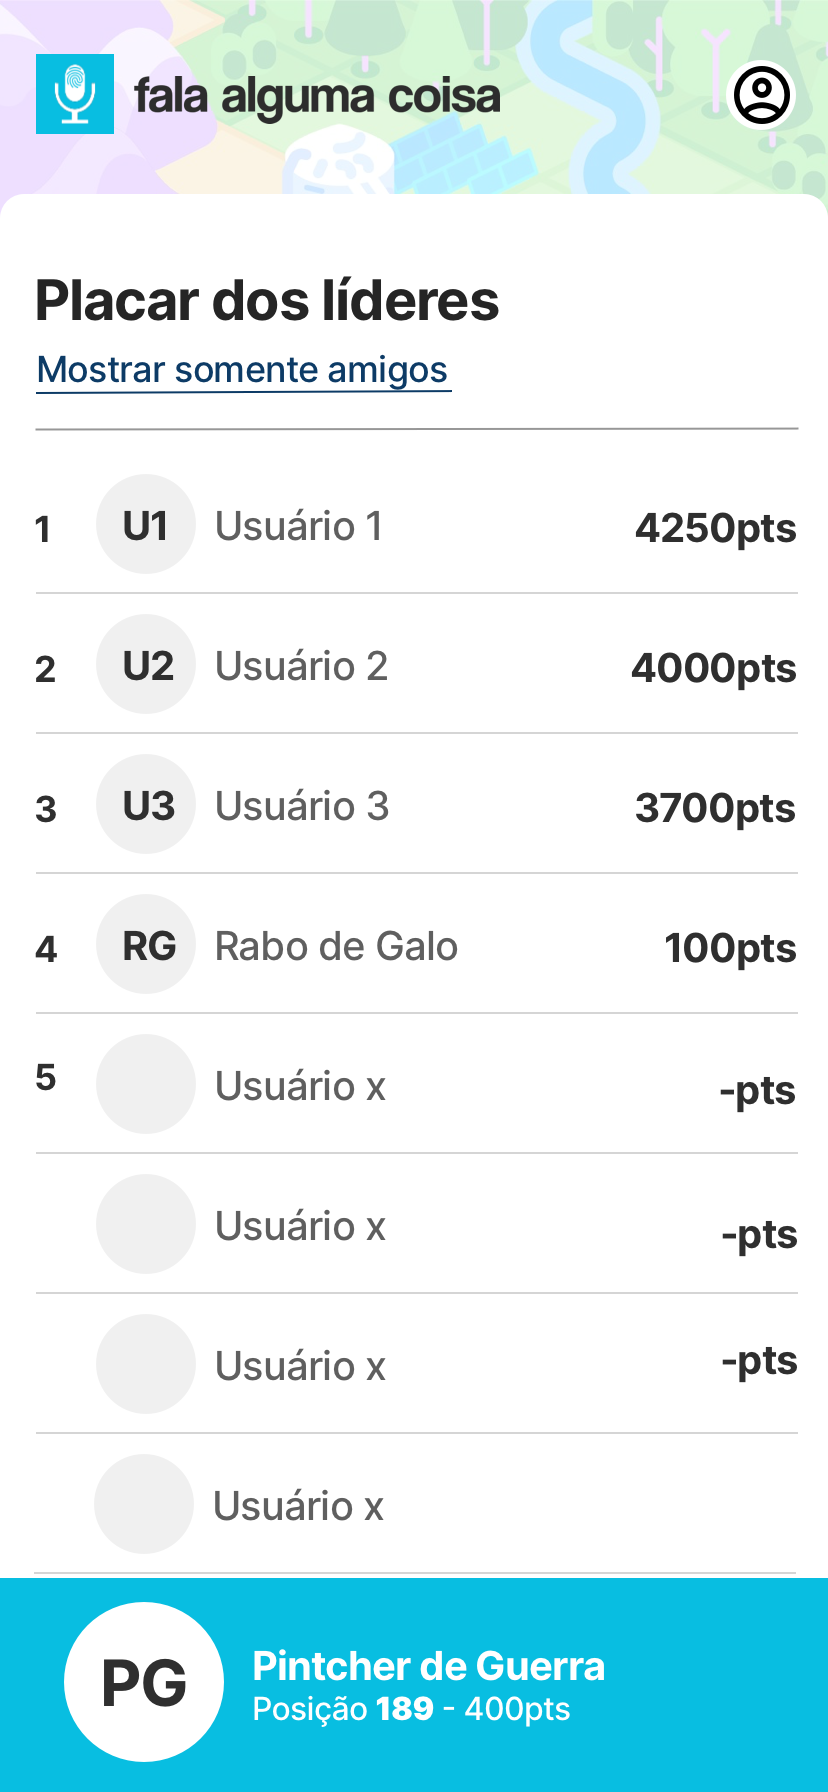
\includegraphics[width=.9\linewidth]{images/app/leaderboard/GeneralRanking.png}}
      \caption{General Leaderboard}
      \label{fig:falealgumacoisa-leaderboard-page-design-general}
    \end{subfigure}%
    \begin{subfigure}{.5\textwidth}
      \centering
      \frame{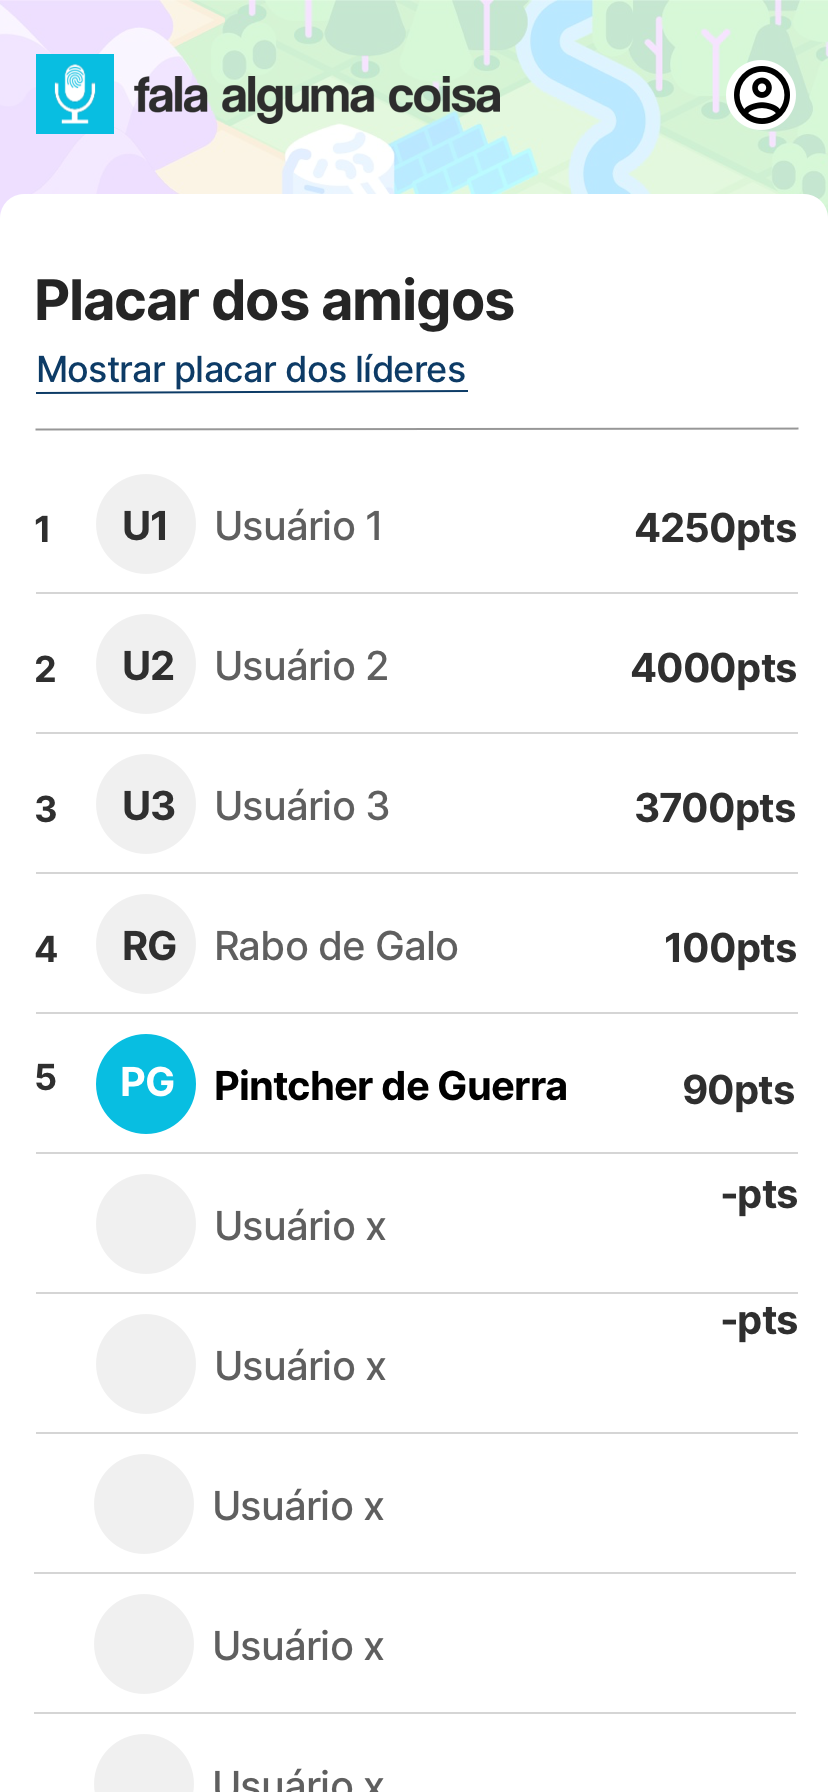
\includegraphics[width=.9\linewidth]{images/app/leaderboard/FriendsRanking.png}}
      \caption{Friends Leaderboard}
      \label{fig:falealgumacoisa-leaderboard-page-design-friend}
    \end{subfigure}
    \caption*{Source: Author}
    \label{fig:falealgumacoisa-leaderboard-page-design}
\end{figure}

\subsubsection{Friends}

The ability to add and track (follow) friends is possible with the layouts described below. If the contributor knows the nickname of his friend, he can search for his friends using the Search Friends page (seen in figure \ref{fig:falealgumacoisa-friends-page-design-search}). The results return in the same page below the search input field (figure \ref{fig:falealgumacoisa-friends-page-design-results}), as a list of users. To add a friend, it is as simple as clicking the "Seguir" button in the right corner of the result list. This click toggles the button with a "Seguindo" text. If this new state is clicked, the friend is removed.

\begin{figure}[ht]
    \centering
    \caption{Fale Alguma Coisa Friends Page designs}
    \begin{subfigure}{.5\textwidth}
      \centering
      \frame{
\includegraphics[width=.9\linewidth]{images/app/friends/FriendsSearch_1.0.png}}
      \caption{Search for friends}
      \label{fig:falealgumacoisa-friends-page-design-search}
    \end{subfigure}%
    \begin{subfigure}{.5\textwidth}
      \centering
      \frame{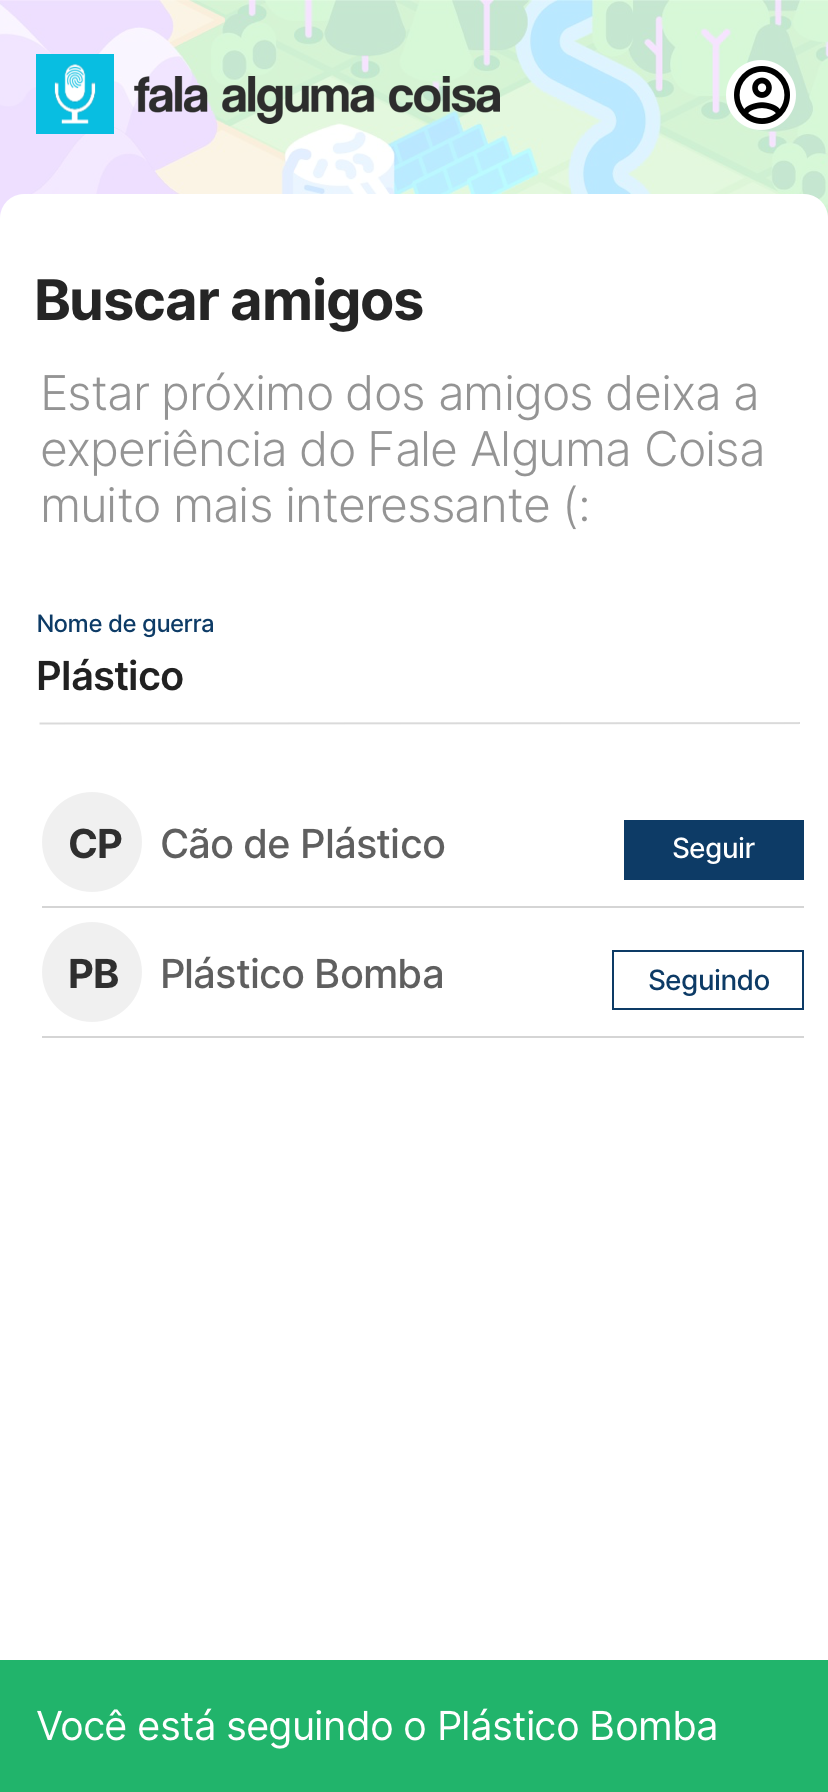
\includegraphics[width=.9\linewidth]{images/app/friends/FriendsSearch_1.3.png}}
      \caption{Search friends results}
      \label{fig:falealgumacoisa-friends-page-design-results}
    \end{subfigure}
    \caption*{Source: Author}
    \label{fig:falealgumacoisa-friends-page-design}
\end{figure}

\subsubsection{Refer Friends}

To earn more contribution points, the citizen scientist can also refer new friends using the Refer friends page. The mobile version of this page is illustrated in figure \ref{fig:falealgumacoisa-refer-page-design}, and has one button "Compartilhar", which enables the mobile sharing functionality. The link shared redirects to a registration page, and both users get 100 points after the registration of the reffered user.

\begin{figure}[ht]
    \centering
    \caption{Fale Alguma Coisa Refer Friends Page design}
    \frame{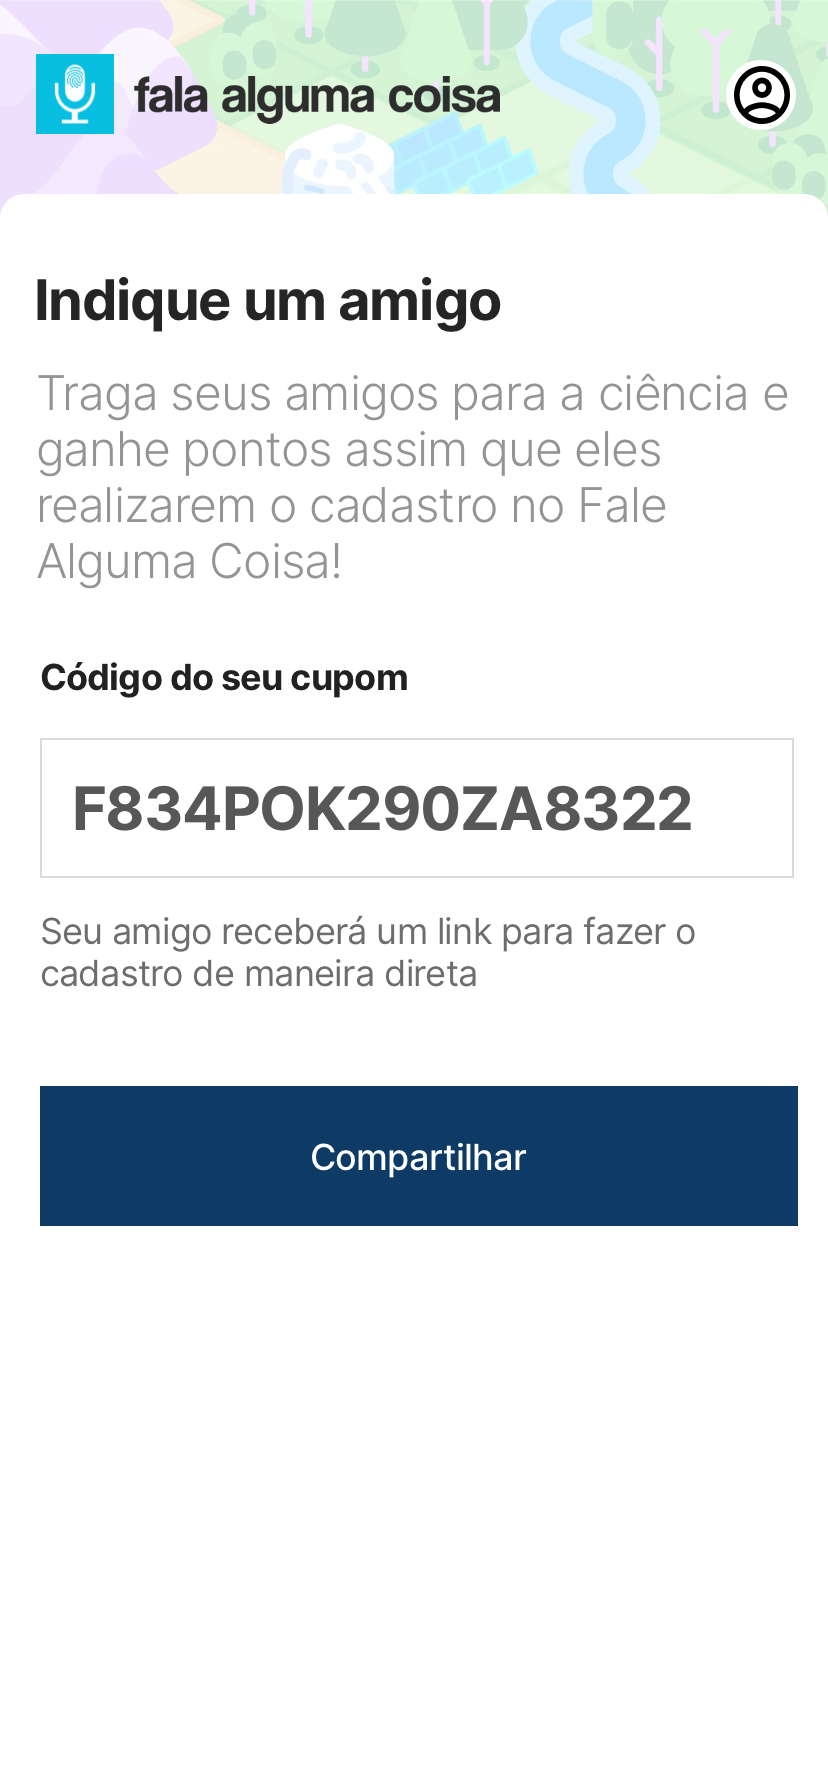
\includegraphics[width=\linewidth/2]{images/app/friends/Search_Friend_1.0.png}}
    \caption*{Source: Author}
    \label{fig:falealgumacoisa-refer-page-design}
\end{figure}

\subsubsection{Login and Registration}

The login and registration pages include essential features to the application: the ability to identify the user and maintain a history of recordings. The figure in \ref{fig:falealgumacoisa-login-page-design} represents a login flow possible to the contributor - using a username and password. It is also possible to use the "social login" through Facebook and Google, identifiable by the respective buttons in the layout.

\begin{figure}[ht]
    \centering
    \caption{Fale Alguma Coisa Login Page designs}
    \begin{subfigure}{.5\textwidth}
      \centering
      \frame{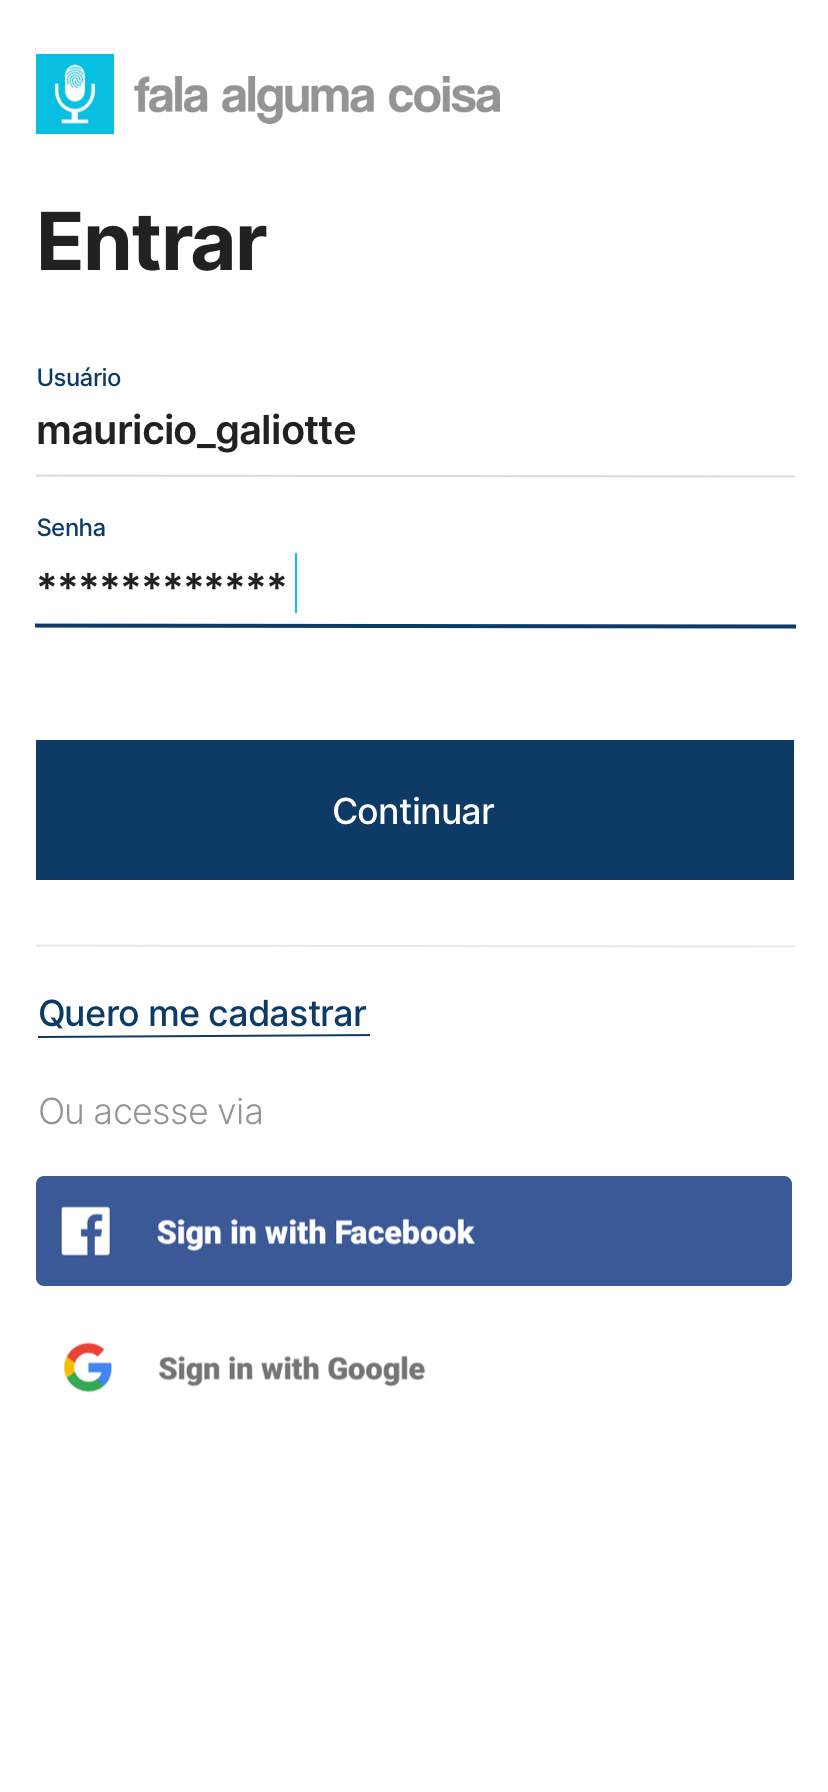
\includegraphics[width=.9\linewidth]{images/app/login/Login2.png}}
      \caption{Login with email and password}
      \label{fig:falealgumacoisa-login-page-design}
    \end{subfigure}%
    \begin{subfigure}{.5\textwidth}
      \centering
      \frame{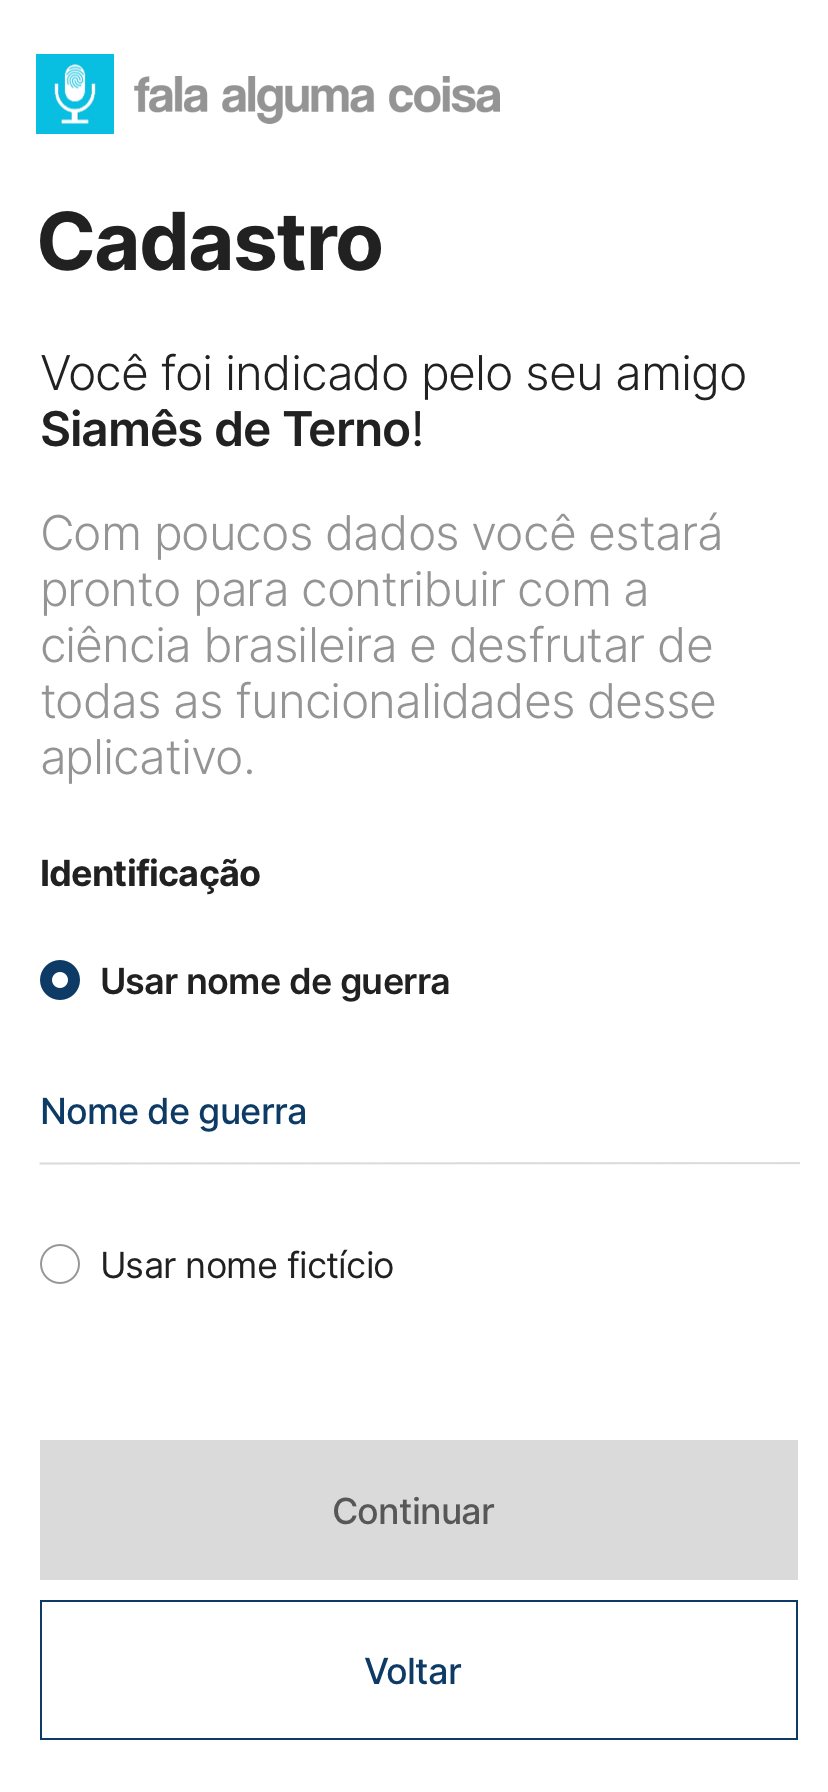
\includegraphics[width=.9\linewidth]{images/app/register/Register1.0.png}}
      \caption{Registration with \textit{pen name} selection}
      \label{fig:falealgumacoisa-registration-page-design-pen-name}
    \end{subfigure}
    \caption*{Source: Author}
    \label{fig:falealgumacoisa-login-and-registration-page-design}
\end{figure}

To register with the Fale Alguma Coisa app, the user must choose his \textit{pen name} (figure \ref{fig:falealgumacoisa-registration-page-design-pen-name}) and add some demographics information (seen in figure \ref{fig:falealgumacoisa-registration-page-design-demographics}. The registration flow can be triggered in two ways, and each have their differences:

\begin{itemize}
    \item Using the "social login" button. In this format, the user authenticates using the social media account and therefore does not need to provide email and password. Subsequent logins should use this method as well.
    \item Using a manual registration button ("Quero me cadastrar"). In addition to the name and demographics, the user must also provide his email and password as a last step (figure \ref{fig:falealgumacoisa-registration-page-design-email-password}).
\end{itemize}

\begin{figure}[ht]
    \centering
    \caption{Fale Alguma Coisa Registration steps designs}
    \begin{subfigure}{.5\textwidth}
      \centering
      \frame{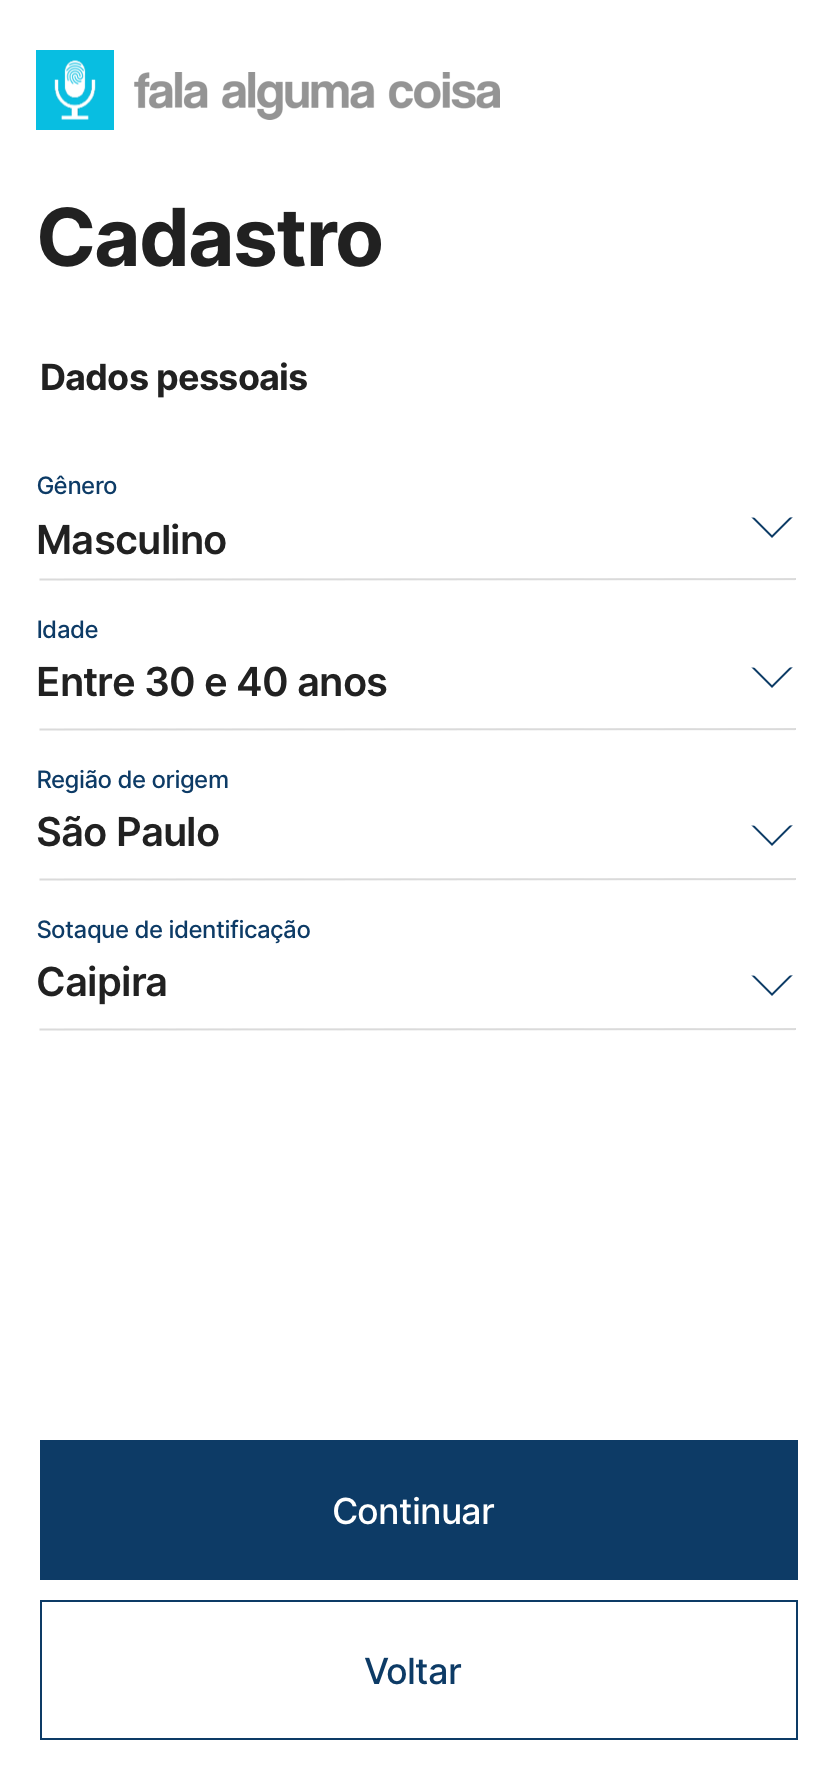
\includegraphics[width=.9\linewidth]{images/app/register/Register2.1.png}}
      \caption{Demographics step}
      \label{fig:falealgumacoisa-registration-page-design-demographics}
    \end{subfigure}%
    \begin{subfigure}{.5\textwidth}
      \centering
      \frame{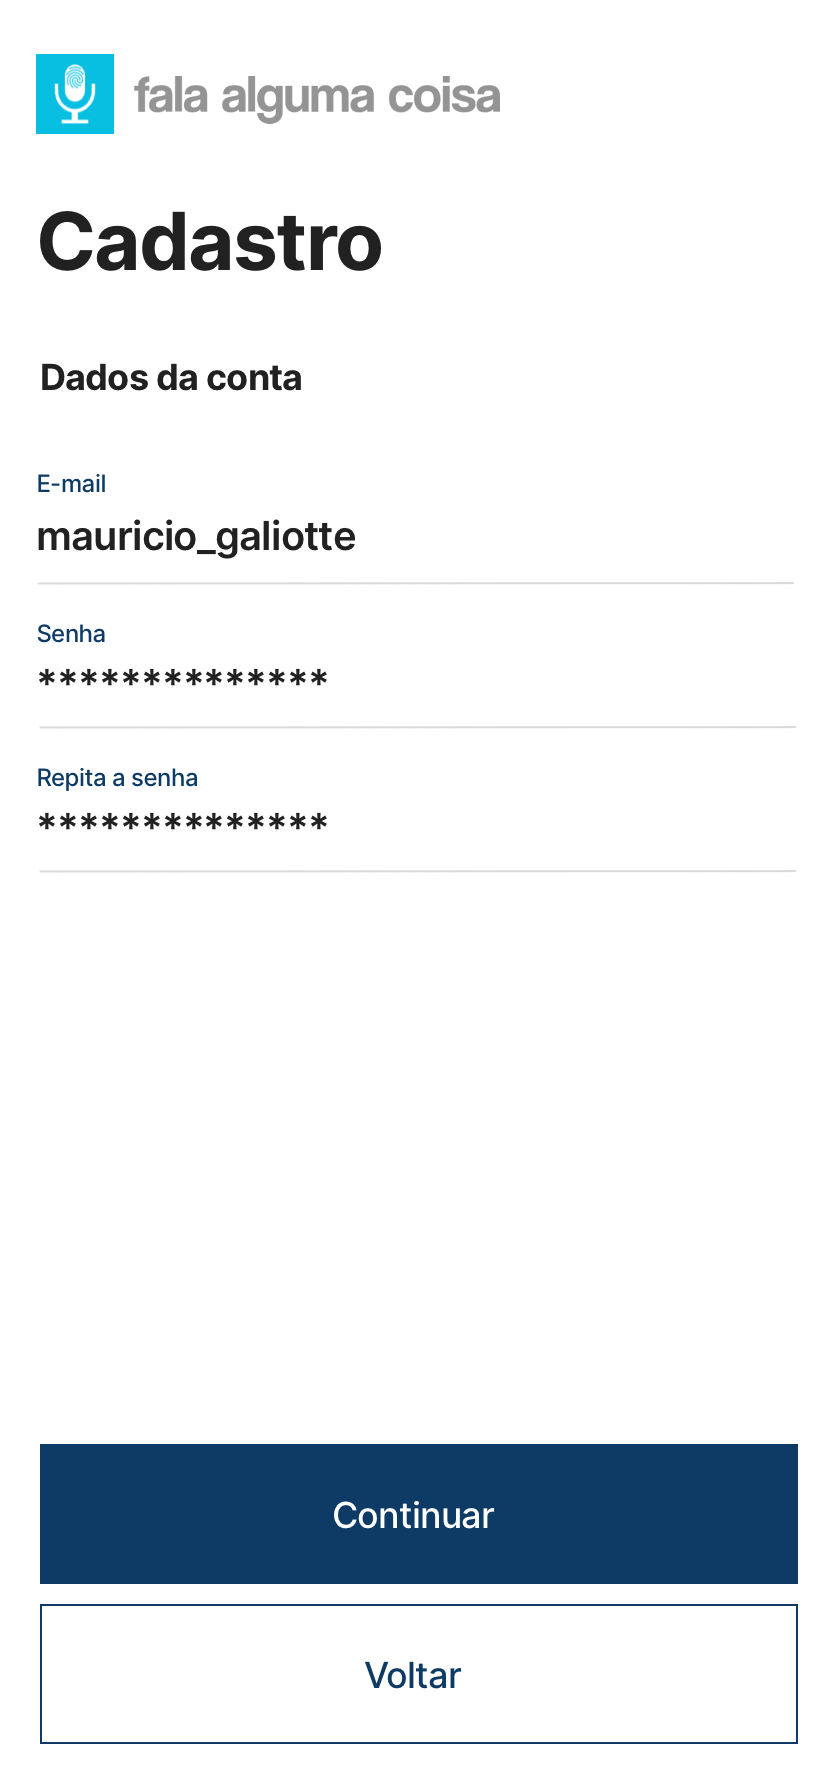
\includegraphics[width=.9\linewidth]{images/app/register/Register3.0.png}}
      \caption{Email and password step}
      \label{fig:falealgumacoisa-registration-page-design-email-password}
    \end{subfigure}
    \caption*{Source: Author}
    \label{fig:falealgumacoisa-registration-page-design}
\end{figure}

\subsubsection{Delete User}

If necessary, the user should be able to delete its user data, while still contributing his voice to the speech corpus. The following figures (\ref{fig:falealgumacoisa-delete-user-data-page-design-1} and \ref{fig:falealgumacoisa-delete-user-data-page-design-2}) include the design of the layout for this deletion flow.

\begin{figure}[ht]
    \centering
    \caption{Fale Alguma Coisa Delete User Data steps designs}
    \begin{subfigure}{.5\textwidth}
      \centering
      \frame{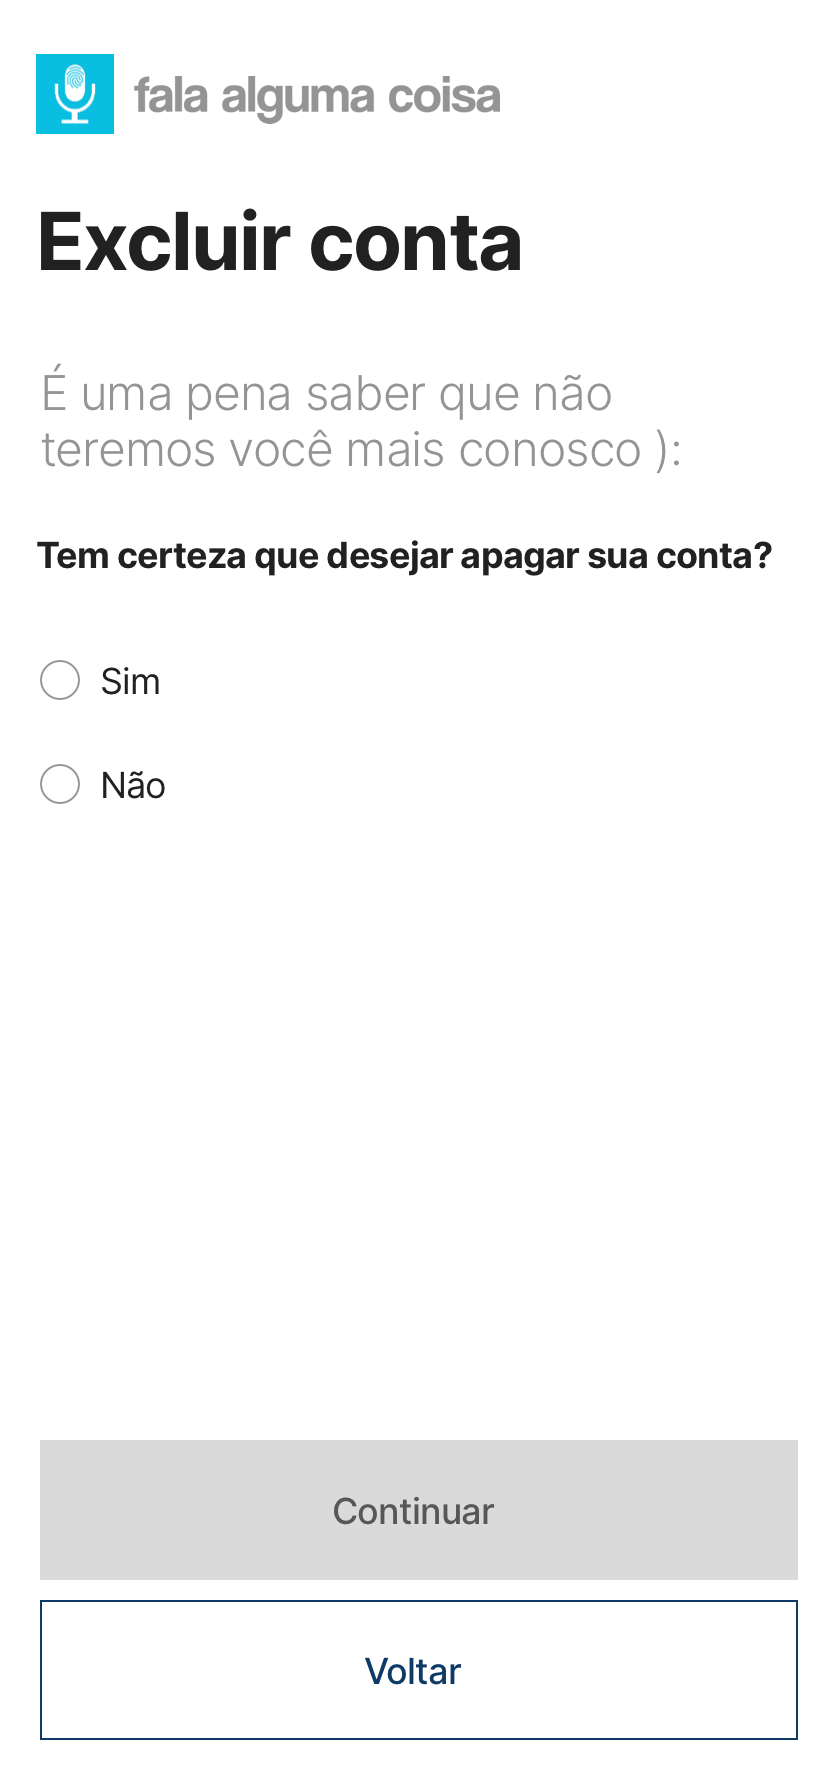
\includegraphics[width=.9\linewidth]{images/app/delete-user/FinishAccount1.0.png}}
      \caption{Deletion confirmation}
      \label{fig:falealgumacoisa-delete-user-data-page-design-1}
    \end{subfigure}%
    \begin{subfigure}{.5\textwidth}
      \centering
      \frame{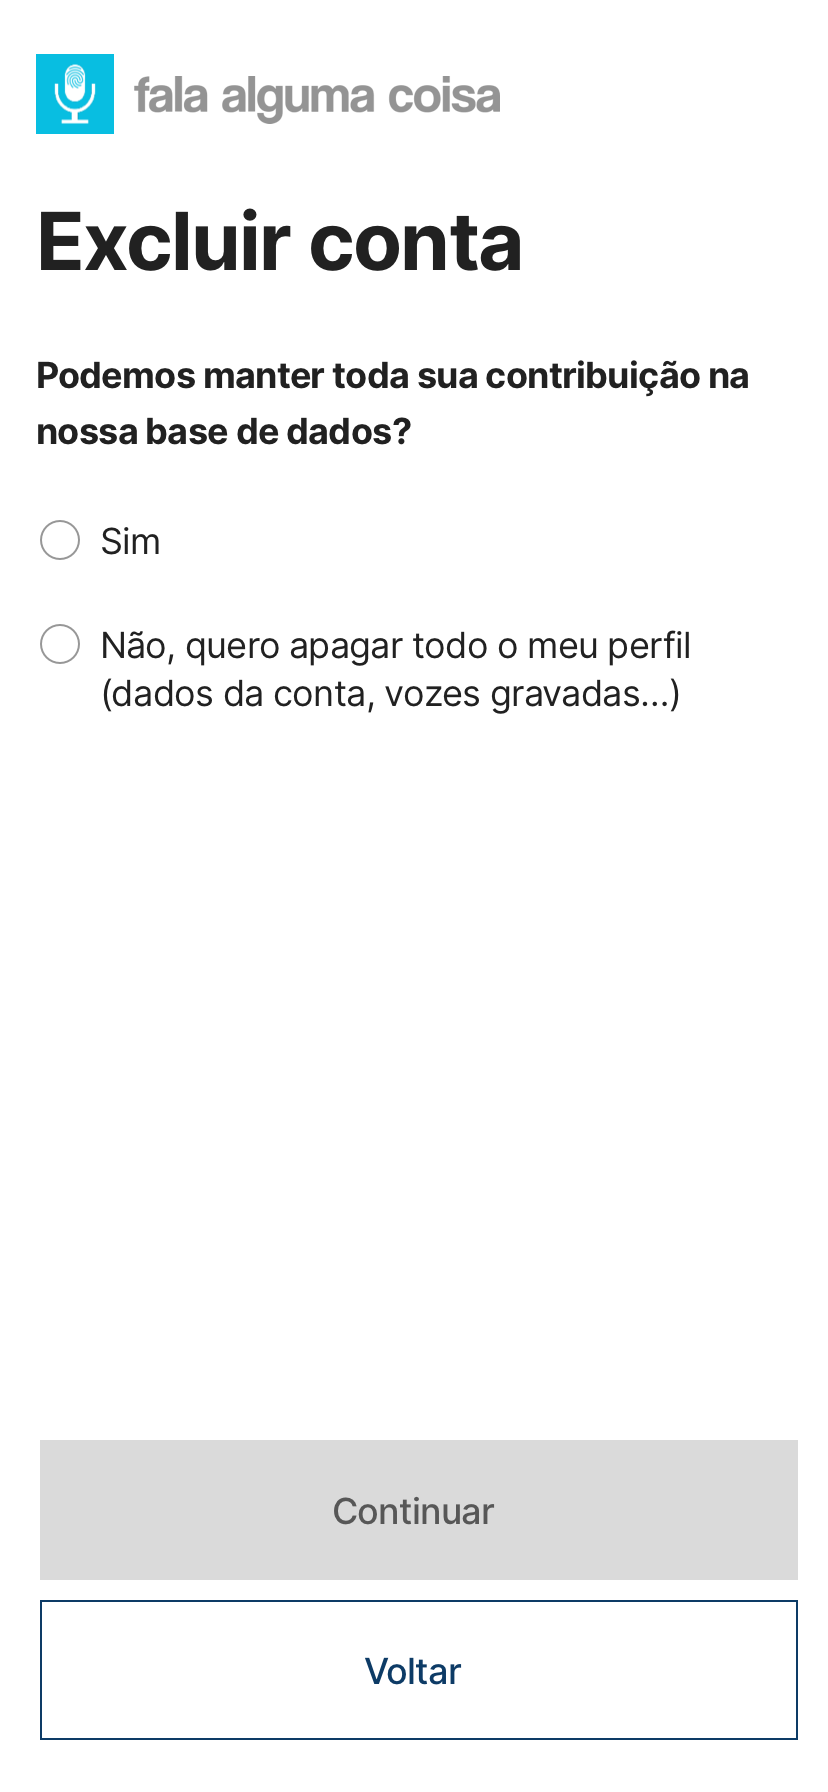
\includegraphics[width=.9\linewidth]{images/app/delete-user/FinishAccount2.0.png}}
      \caption{Scope of deletion}
      \label{fig:falealgumacoisa-delete-user-data-page-design-2}
    \end{subfigure}
    \caption*{Source: Author}
    \label{fig:falealgumacoisa-delete-user-data-page-design}
\end{figure}

\subsubsection{Remaining Implementations}

Refer to Appendix \ref{appendix:user-interface-design} for the remaining implemented user interfaces.

\clearpage
\subsection{Phrase Selection}
\label{sec:app-phrase-selection}

One of the key aspects of the Fale Alguma Coisa application is the ability of explaining science-related trivia. In the process of recording, the contributor may learn small facts about the chosen topic by reading a group of scientific phrases. The following sections will detail the anatomy of a theme, the requirements for selecting a phrase, the phrases source, along with the filtering process.

\subsubsection{Theme Anatomy}

Each group of phrases is entitled "theme". By specification (\ref{srs:uc12} and \ref{srs:uc16}), a theme is composed of 8 phrases: 6 of which must be recorded to finish a theme; allowing up to 2 skips. Figure \ref{fig:falealgumacoisa-phrase-all} illustrates the anatomy of a theme and figure \ref{phrase-skip} displays what happens to a recording group when a phrase is skipped.

\begin{figure}[h]
    \centering
    \caption{Selected phrases of a theme. Out of 8, only 6 are shown to the user.}
    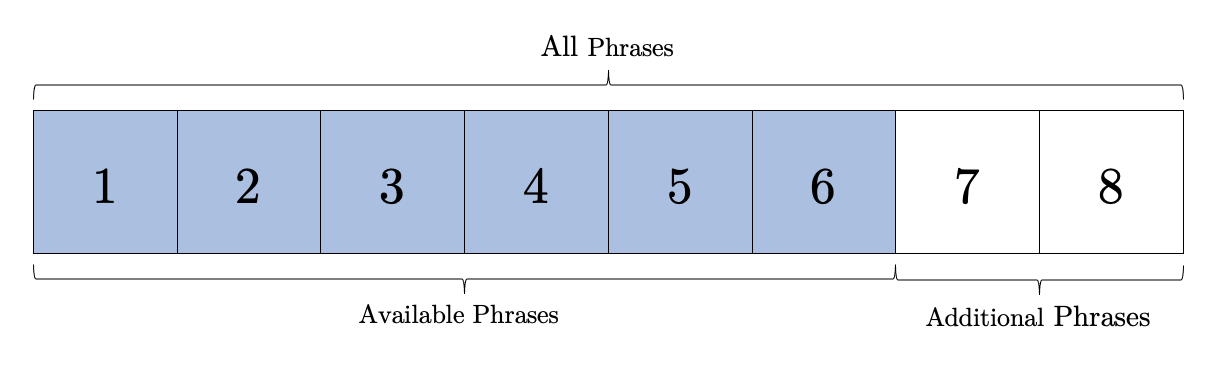
\includegraphics[width=\linewidth]{images/sw-req-spec/phrase-all.png}
    \caption*{Source: Author}
    \label{fig:falealgumacoisa-phrase-all}
\end{figure}

\begin{figure}[h]
    \centering
    \caption{Recorded theme example. The sixth phrase was skipped, thus allowing the recording of the seventh phrase.}
    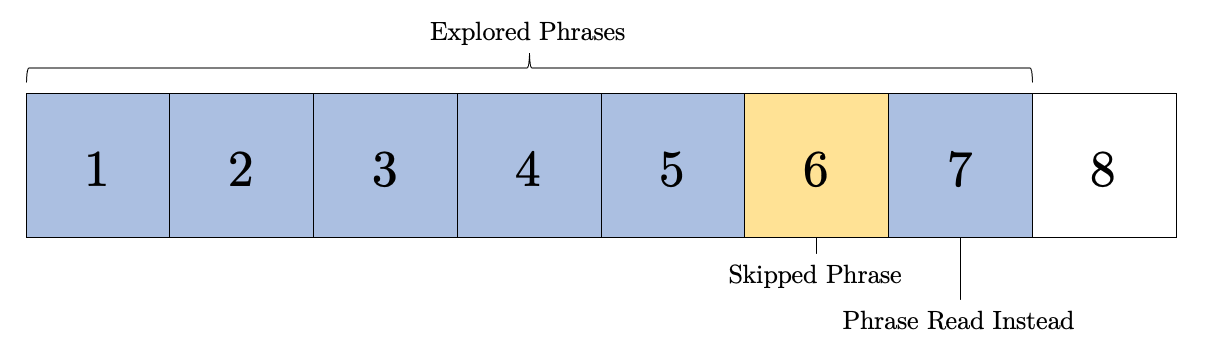
\includegraphics[width=\linewidth]{images/sw-req-spec/phrase-skip.png}
    \caption*{Source: Author}
    \label{fig:falealgumacoisa-phrase-skip}
\end{figure}

\subsubsection{Selection Process}

In addition to the number of phrases per group, the selection process of each phrase must be detailed. This section details such process, therefore necessitating the phrases to adhere to some requirements: 

\begin{enumerate}
    \item the phrase must not contain more than 110 characters, so that it fits within the breakpoints specification of the recording page;
    \item must be related to the theme chosen, to compound the knowledge of the other spoken phrases in the same theme;
    \item must be a fact, or at least reviewed by one or more individuals, so that there is no spread of misinformation;
    \item must be in Portuguese, since it is a Portuguese corpus;
    \item must not use very uncommon words, to facilitate reading;
    \item must be copyright free, for use in the application.
\end{enumerate}

\subsubsection{Phrases Source}

To extract phrases with such requirements, a extensive Portuguese phrases list must be compiled.

\subsubsection{Phrases Filtering}

\begin{table}[h]
    \centering
    \caption{SLR - Filtering of results}
    \begin{tabular}{|c|c|}
        \hline Step & Results \\ \hline
        Full extraction & 157 \\ \hline
        Length limitation & 23 \\ \hline
        Themes filtering & 14 \\ \hline
        Reviews & 14 \\ \hline
        Common words & 14 \\ \hline
    \end{tabular}
    \caption*{Source: Author}
    \label{tab:filtering}
\end{table}

\subsection{Development}
\label{sec:app-development}

This section details the development process of the Fale Alguma Coisa app.

\subsubsection{Web app}

To allow easier access to the voice recording app, a web-based application will be developed. This factor positively influences the capacity of the app to update over time, when compared to an application developed in a native environment. It also enables users over mobile and desktop to access the same application, and although the layout may have to be redesigned, most logic is reused.

\subsubsection{Mobile First}

The design will use a mobile first approach, to ensure the user flow will be optimized when he is using a mobile device. The desktop flow will be designed and developed afterwards.

\subsubsection{Tools Selection}

To develop the application, a selection of tools was made. The table \ref{tab:tools-selection} details the selected tools and explains each choice.

\begin{table}[h]
    \centering
    \begin{tabular}{|c|c|c|}
        \hline Category & Selection & Explanation \\
        \hline Design & Zeplin & Easy sharing  \\ 
        \hline Design &  & access \\ 
        \hline  & access & access \\ 
        \hline Christmas Audubom Birdwatch & access & access \\ \hline 
    \end{tabular}
    \caption{Contribution for online citizen science projects}
    \label{tab:tools-selection}
\end{table}


\section{General Public Submission}
\label{sec:proposal-public-submission}

\section{Data Analysis}
\label{sec:proposal-data-analysis}

\section{Data Publication}
\label{sec:proposal-data-publication}